\documentclass[12pt,a4paper]{article}

\usepackage[a4paper,margin=1in]{geometry}
\setlength{\headheight}{14.5pt}
\addtolength{\topmargin}{-2.5pt}
\usepackage{graphicx}
\graphicspath{{../output_plots/}}
\usepackage{booktabs}
\usepackage{amsmath,amssymb}
\usepackage{float}
\usepackage{xurl}
\usepackage{hyperref}
\usepackage{xcolor}
\usepackage{listings}
\usepackage{enumitem}
\usepackage{fancyhdr}
\usepackage{longtable}

\hypersetup{colorlinks=true,linkcolor=blue,urlcolor=blue}

\pagestyle{fancy}
\fancyhf{}
\lhead{ICS1512}
\rhead{Machine Learning Algorithms Laboratory}
\cfoot{\thepage}

\lstset{
language=Python,
basicstyle=\ttfamily\small,
numbers=left,
frame=single,
breaklines=true,
showstringspaces=false
}

\begin{document}

\noindent
\begin{tabular}{|p{3.8cm}|p{11.2cm}|}
\hline
\textbf{Experiment No.} & 8 \\ \hline
\textbf{Experiment Title} & Clustering Human Activity Recognition Data using K-Means, DBSCAN, and Hierarchical Clustering\footnotemark \\ \hline
\textbf{Student Name} & Danusu K \\ \hline
\textbf{Register Number} & 3122247001013 \\ \hline
\textbf{Faculty} & Dr. Poreddy Ajay Kumar Reddy \\ \hline
\textbf{Submission Date} & \today \\ \hline
\end{tabular}
\footnotetext{\textbf{GitHub Repository: }\url{https://github.com/Danush-k/Machine-Learning}}

\section{Objective}
\begin{itemize}
\item To implement and comparatively analyze three unsupervised clustering algorithms — \textbf{K-Means}, \textbf{DBSCAN}, and \textbf{Hierarchical Agglomerative Clustering (HAC)} — on the \textbf{UCI Human Activity Recognition (HAR) Using Smartphones} dataset.
\item To select the optimal number of clusters for K-Means using the \textbf{Elbow Method} (WCSS) and \textbf{Silhouette Score}.
\item To tune DBSCAN's neighborhood radius $\epsilon$ and minimum-points threshold minPts using a \textbf{k-distance graph} and systematic grid search.
\item To compare \textbf{single, complete, average, and Ward} linkage criteria for Hierarchical Clustering and visualize the resulting dendrograms.
\item To visualize clusters in 2D using \textbf{PCA} and \textbf{t-SNE}, and rigorously evaluate all three models using internal validation metrics (Silhouette, Davies-Bouldin, Calinski-Harabasz) and external validation against ground-truth activity labels (Adjusted Rand Index, Normalized Mutual Information).
\end{itemize}

\section{Problem Statement}
Wearable and smartphone-based sensors generate continuous, high-dimensional, unlabeled motion data in real-world deployments. While supervised classifiers can recognize activities when labeled training data is available, many practical scenarios (new users, new sensor placements, unsupervised anomaly detection) require discovering the underlying activity structure directly from unlabeled accelerometer/gyroscope feature vectors. The UCI HAR dataset provides 561 time- and frequency-domain features extracted from tri-axial smartphone sensor windows for 30 volunteers performing 6 activities. This experiment investigates whether unsupervised clustering algorithms — differing fundamentally in their structural assumptions (centroid-based, density-based, and hierarchical/variance-based) — can recover a meaningful activity structure from this feature space without access to labels, and characterizes each algorithm's strengths, failure modes, and sensitivity to hyperparameters.

\section{Theoretical Background}

\subsection{K-Means Clustering}
K-Means partitions $N$ observations into $k$ clusters by minimizing the within-cluster sum of squares (WCSS):
\begin{equation}
J = \sum_{i=1}^{k} \sum_{\mathbf{x} \in C_i} \lVert \mathbf{x} - \boldsymbol{\mu}_i \rVert^2
\end{equation}
where $\boldsymbol{\mu}_i$ is the centroid of cluster $C_i$. The algorithm alternates between (1) assigning each point to its nearest centroid and (2) recomputing centroids as the mean of assigned points, until convergence (Lloyd's algorithm). K-Means assumes roughly convex, isotropic, similarly-sized clusters.

\subsection{DBSCAN}
Density-Based Spatial Clustering of Applications with Noise identifies clusters as dense, connected regions separated by regions of low density, using two parameters: $\epsilon$ (neighborhood radius) and $\text{minPts}$ (minimum neighbors for a core point). A point $\mathbf{p}$ is a \textbf{core point} if $|N_\epsilon(\mathbf{p})| \ge \text{minPts}$; a \textbf{border point} lies within $\epsilon$ of a core point but has fewer than minPts neighbors itself; all other points are labeled \textbf{noise}. Clusters are formed by density-connecting core points. Unlike K-Means, DBSCAN does not require the number of clusters to be specified a priori and can discover arbitrarily-shaped clusters, but it is sensitive to $\epsilon$/minPts and struggles when clusters have varying density.

\subsection{Hierarchical Agglomerative Clustering (HAC)}
HAC builds a hierarchy of nested clusters bottom-up: each point starts as its own cluster, and the two closest clusters are iteratively merged until one cluster remains, producing a \textbf{dendrogram}. The merge criterion (\textbf{linkage}) determines behavior:
\begin{align}
\text{Single: } & d(A,B) = \min_{a \in A, b \in B} \lVert a - b \rVert \\
\text{Complete: } & d(A,B) = \max_{a \in A, b \in B} \lVert a - b \rVert \\
\text{Average: } & d(A,B) = \frac{1}{|A||B|}\sum_{a \in A}\sum_{b \in B} \lVert a - b \rVert \\
\text{Ward: } & d(A,B) = \frac{|A||B|}{|A|+|B|} \lVert \boldsymbol{\mu}_A - \boldsymbol{\mu}_B \rVert^2
\end{align}
Single linkage is prone to \textit{chaining} (a sequence of close points bridges otherwise distinct clusters); Ward's linkage minimizes the increase in total within-cluster variance at each merge, typically producing the most balanced partitions.

\section{Dataset Description \& Preprocessing}
\begin{longtable}{|p{5.5cm}|p{8.5cm}|}
\hline
\textbf{Attribute} & \textbf{Specification} \\ \hline
\endhead
Dataset Name & Human Activity Recognition Using Smartphones (UCI HAR Dataset) \\ \hline
Dataset Source & UCI Machine Learning Repository \\ \hline
Volunteers & 30 subjects, aged 19--48 \\ \hline
Sensors & Waist-mounted smartphone, 3-axis accelerometer + gyroscope @ 50Hz \\ \hline
Windowing & 2.56s windows, 128 readings/window, 50\% overlap \\ \hline
Total Samples & 10,299 windows (7,352 train + 2,947 test; merged for unsupervised analysis) \\ \hline
Number of Features & 561 time- and frequency-domain features \\ \hline
Target Classes & 6 (WALKING, WALKING\_UPSTAIRS, WALKING\_DOWNSTAIRS, SITTING, STANDING, LAYING) \\ \hline
Missing Values & 0 (complete, pre-cleaned UCI release) \\ \hline
Preprocessing & Feature-wise z-score standardization (\texttt{StandardScaler}) on the merged corpus \\ \hline
Dimensionality Reduction & PCA retaining $\ge 90\%$ cumulative variance (65 components) used as the working feature space for all clustering algorithms; PCA/t-SNE to 2D used only for visualization \\ \hline
\end{longtable}

\begin{figure}[H]
\centering
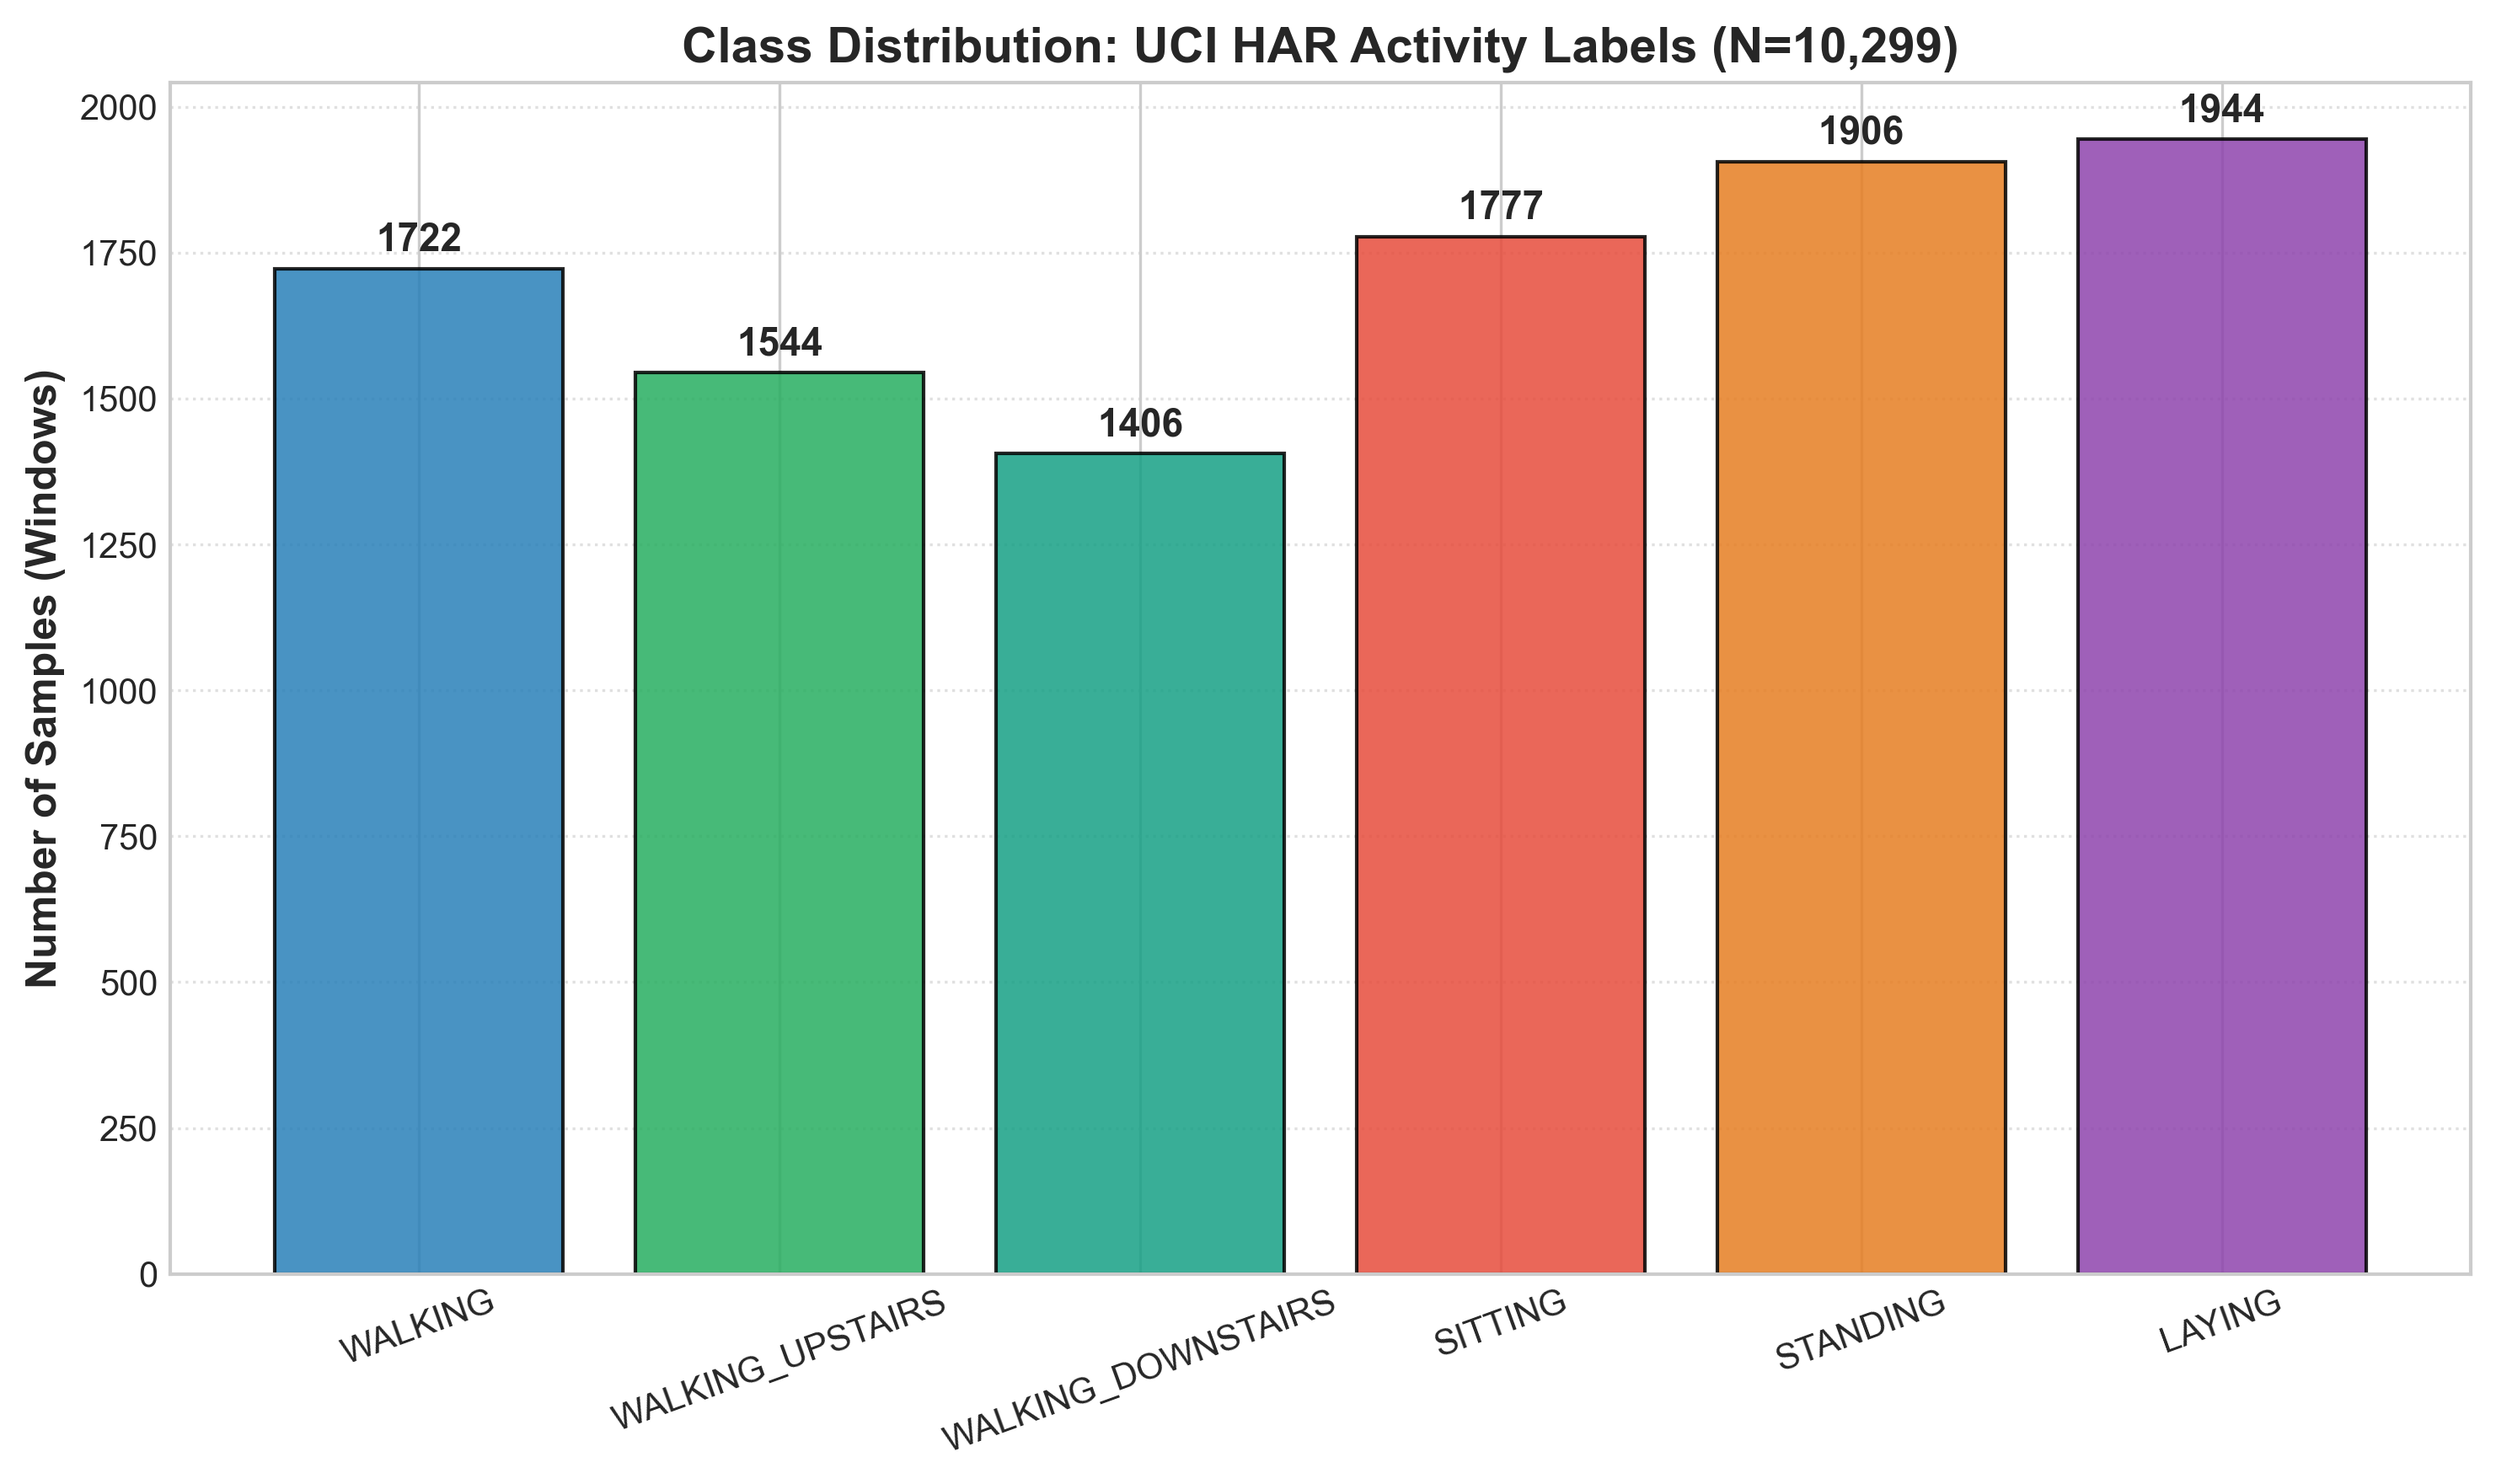
\includegraphics[width=0.75\linewidth]{01_activity_class_distribution.png}
\caption{Class Distribution of the 6 HAR Activity Labels ($N=10{,}299$).}
\end{figure}

\section{PCA Analysis: Scree Plot \& Dimensionality Reduction}
PCA was performed on the standardized 561-dimensional feature space. Table~\ref{tab:pca_variance} presents the eigenvalues and explained variance of the leading components.

\begin{table}[H]
\centering
\caption{PCA Variance Explained \& Scree Decomposition (First 10 of 561 Components)}
\label{tab:pca_variance}
\begin{tabular}{ccc}
\toprule
\textbf{PC \#} & \textbf{Explained Var (\%)} & \textbf{Cumulative Var (\%)} \\
\midrule
PC1 & 50.74\% & 50.74\% \\
PC2 & 6.24\% & 56.98\% \\
PC3 & 2.69\% & 59.67\% \\
PC4 & 2.45\% & 62.12\% \\
PC5 & 1.89\% & 64.01\% \\
PC6 & 1.63\% & 65.64\% \\
PC7 & 1.41\% & 67.06\% \\
PC8 & 1.22\% & 68.27\% \\
PC9 & 0.99\% & 69.26\% \\
PC10 & 0.95\% & 70.21\% \\
\textbf{PC65} & --- & \textbf{90.05\% (Chosen Cutoff)} \\
PC104 & --- & 95.02\% \\
PC182 & --- & 99.01\% \\
\bottomrule
\end{tabular}
\end{table}

\noindent
\textbf{Justification:} A cumulative variance target of \textbf{90\%} was selected for the clustering feature space, retained by the first \textbf{65} of 561 components — an \textbf{88.4\% reduction in dimensionality}. This mitigates the curse of dimensionality for the Euclidean-distance-based algorithms used here (K-Means, DBSCAN, HAC) while preserving the dominant structure of the data. PC1 alone captures \textbf{50.74\%} of total variance and, as shown below, corresponds almost entirely to the separation between dynamic and static activities.

\begin{figure}[H]
\centering
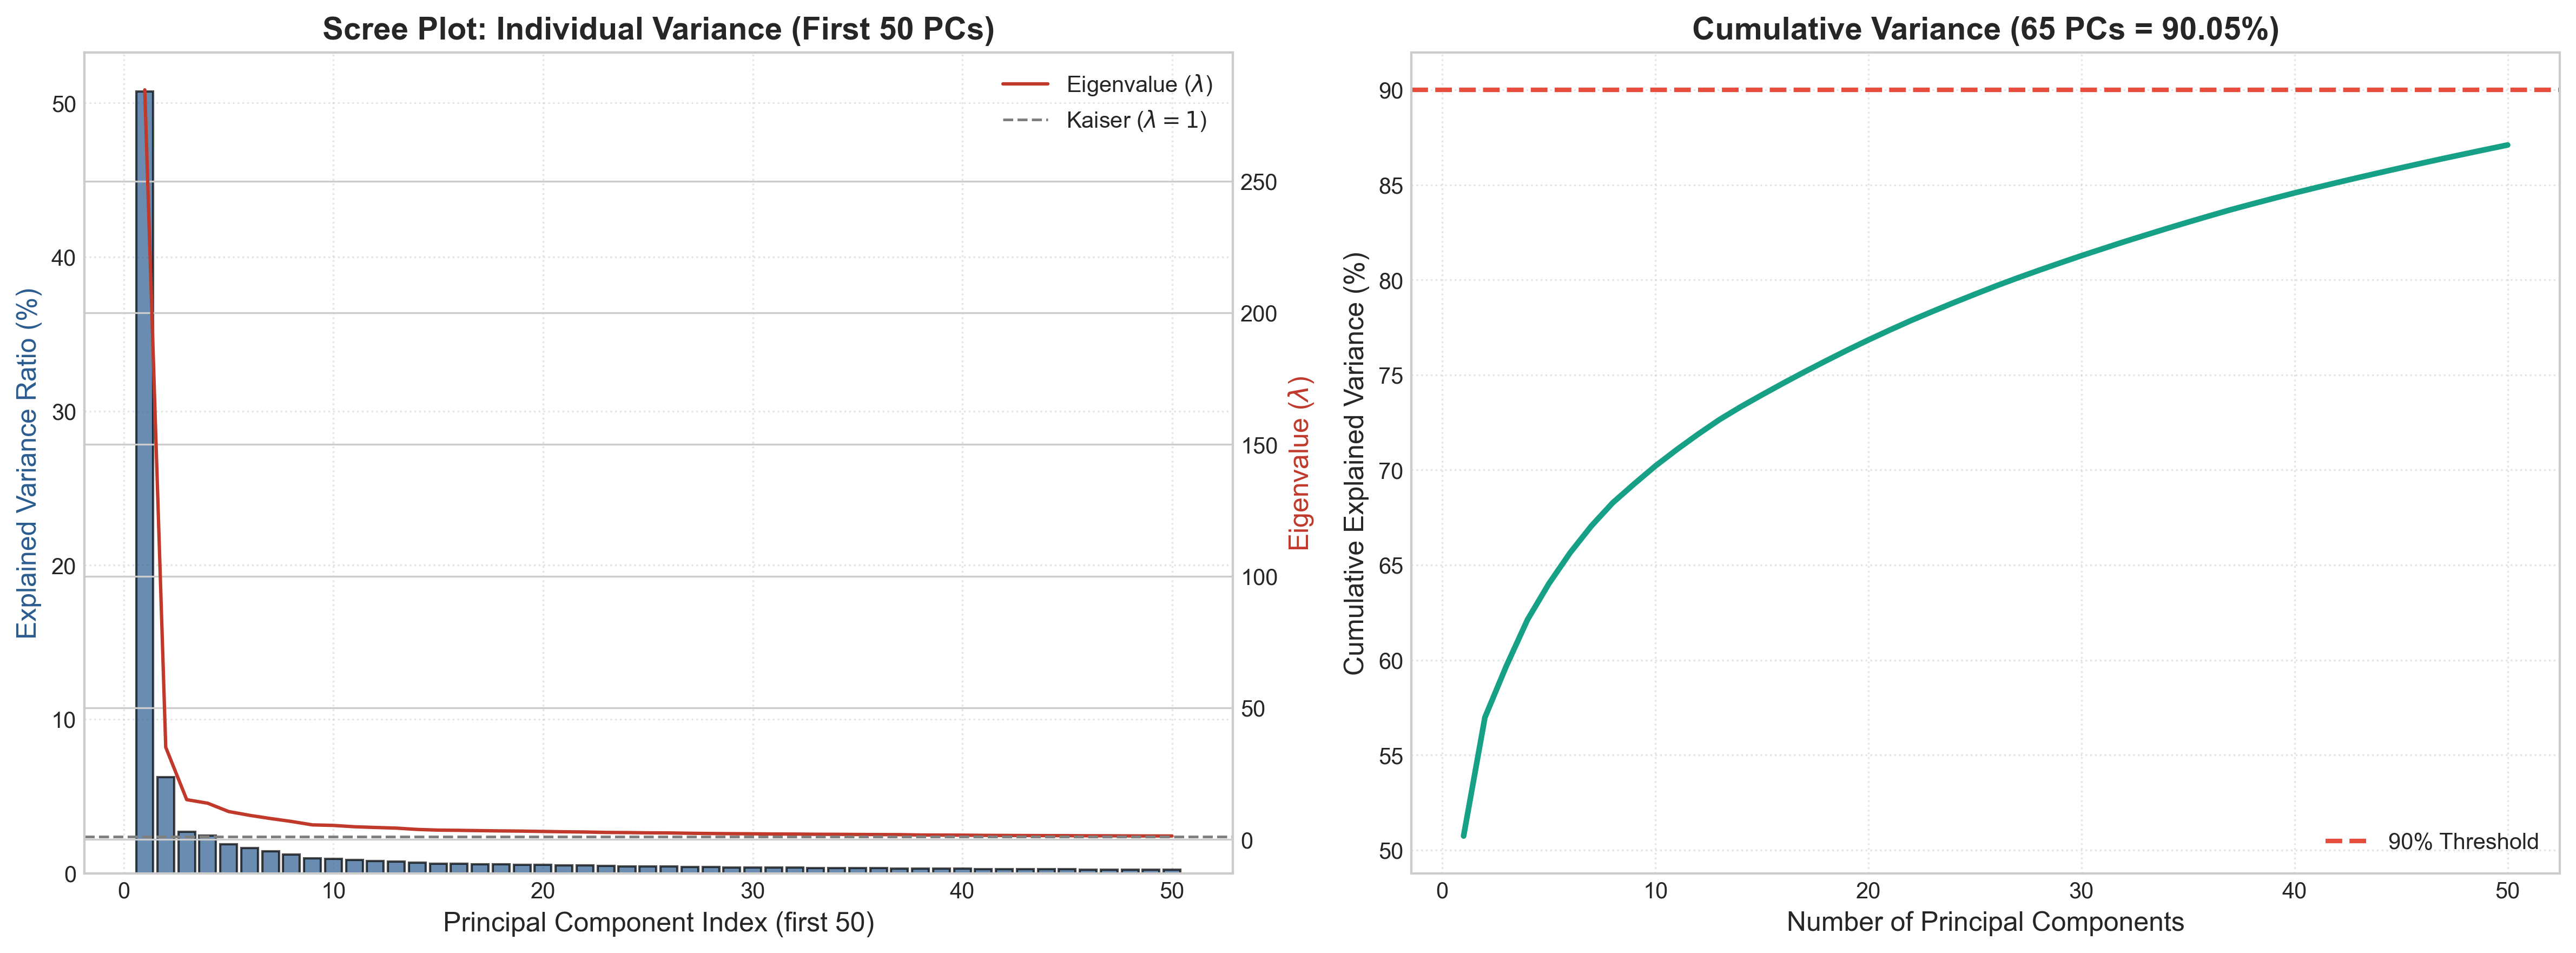
\includegraphics[width=0.98\linewidth]{02_pca_scree_and_cumulative_variance.png}
\caption{Scree Plot (first 50 components) and Cumulative Explained Variance with 90\% Cutoff.}
\end{figure}

\section{Model A: K-Means Clustering}

\subsection{Elbow Method \& Silhouette Analysis}
K-Means was fit for $k=2,\dots,8$ using \texttt{k-means++} initialization ($n\_init=10$). Table~\ref{tab:kmeans_elbow} reports WCSS, Silhouette Score, and external agreement (ARI, NMI) against the true activity labels at each $k$.

\begin{table}[H]
\centering
\caption{K-Means Elbow Method Results}
\label{tab:kmeans_elbow}
\begin{tabular}{cccccc}
\toprule
\textbf{k} & \textbf{WCSS (Inertia)} & \textbf{Silhouette} & \textbf{Davies-Bouldin} & \textbf{ARI} & \textbf{NMI} \\
\midrule
\textbf{2} & 2,697,926.8 & \textbf{0.4366} & \textbf{0.9611} & 0.3296 & \textbf{0.5455} \\
3 & 2,346,425.1 & 0.3519 & 1.5974 & 0.3318 & 0.5184 \\
4 & 2,207,133.3 & 0.1823 & 2.0573 & 0.2985 & 0.4693 \\
5 & 2,081,104.6 & 0.1597 & 2.1379 & 0.2912 & 0.4604 \\
6 & 2,003,581.4 & 0.1400 & 2.0675 & 0.4201 & 0.5597 \\
7 & 1,947,312.3 & 0.1184 & 2.2854 & 0.4155 & 0.5456 \\
8 & 1,892,509.0 & 0.1017 & 2.2515 & \textbf{0.4307} & 0.5542 \\
\bottomrule
\end{tabular}
\end{table}

\noindent
\textbf{Selected $k$:} WCSS decays smoothly with no sharp elbow, but Silhouette Score peaks unambiguously at \textbf{$k=2$} and decreases monotonically thereafter, so $k=2$ is selected as the internally-optimal configuration — corresponding to the coarse \textit{dynamic-vs-static} activity split. Interestingly, $k=6$ (matching the true activity count) is \textit{not} internally optimal but achieves the best external agreement among low-$k$ candidates (ARI=0.4201), since it begins resolving individual activities nested within each super-cluster.

\begin{figure}[H]
\centering
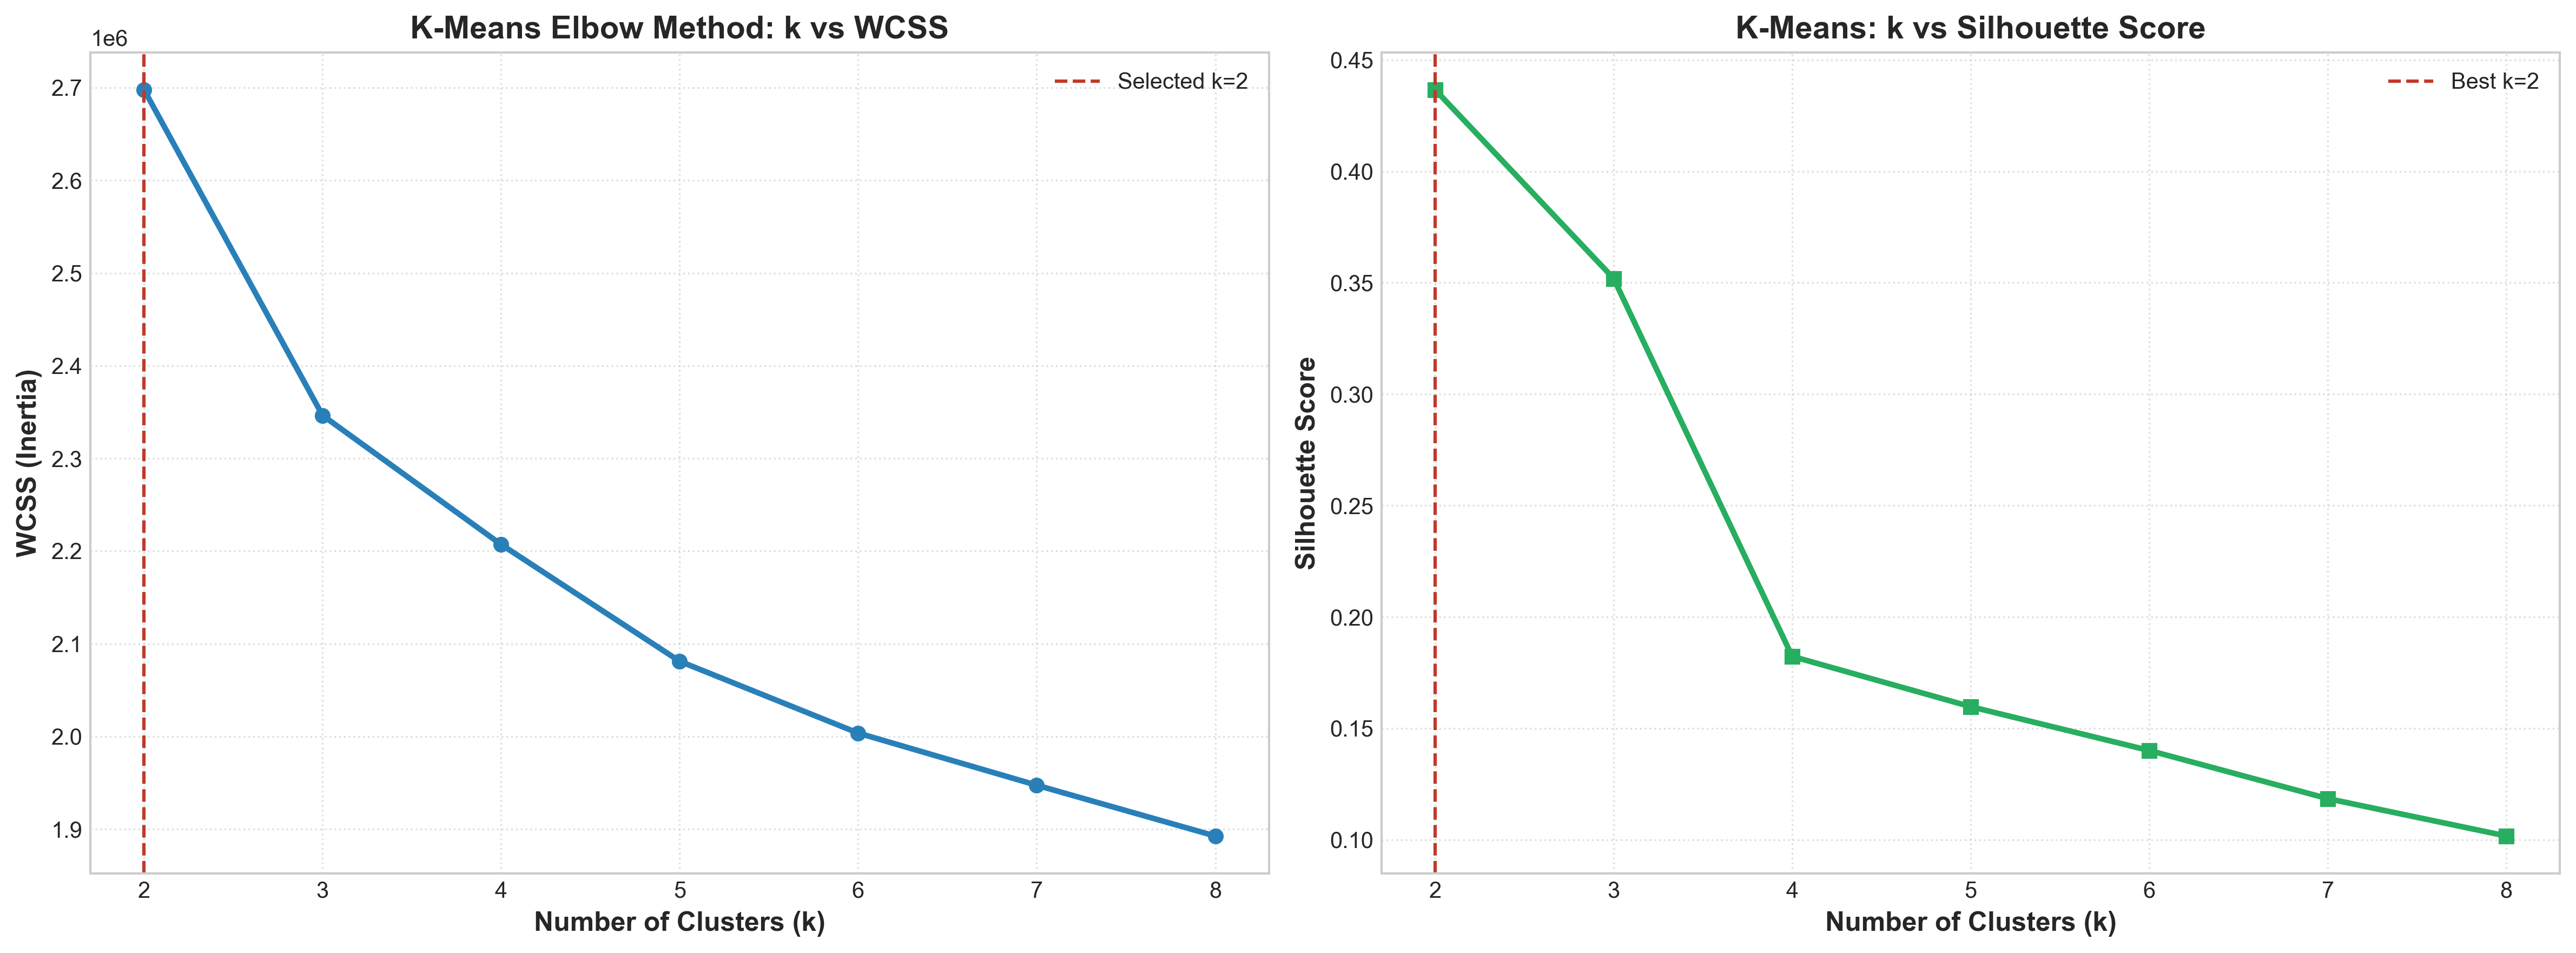
\includegraphics[width=0.98\linewidth]{03_kmeans_elbow_and_silhouette.png}
\caption{K-Means Elbow Curve (k vs WCSS) and Silhouette Curve (k vs Silhouette Score).}
\end{figure}

\section{Model B: DBSCAN}

\subsection{k-Distance Graph \& (eps, minPts) Grid Search}
The 10-NN distance graph (Figure~\ref{fig:kdist}) guides candidate $\epsilon$ values from percentiles of the knee region; minPts was swept over $\{5,10,15,20\}$. Table~\ref{tab:dbscan_grid} reports selected grid points.

\begin{figure}[H]
\centering
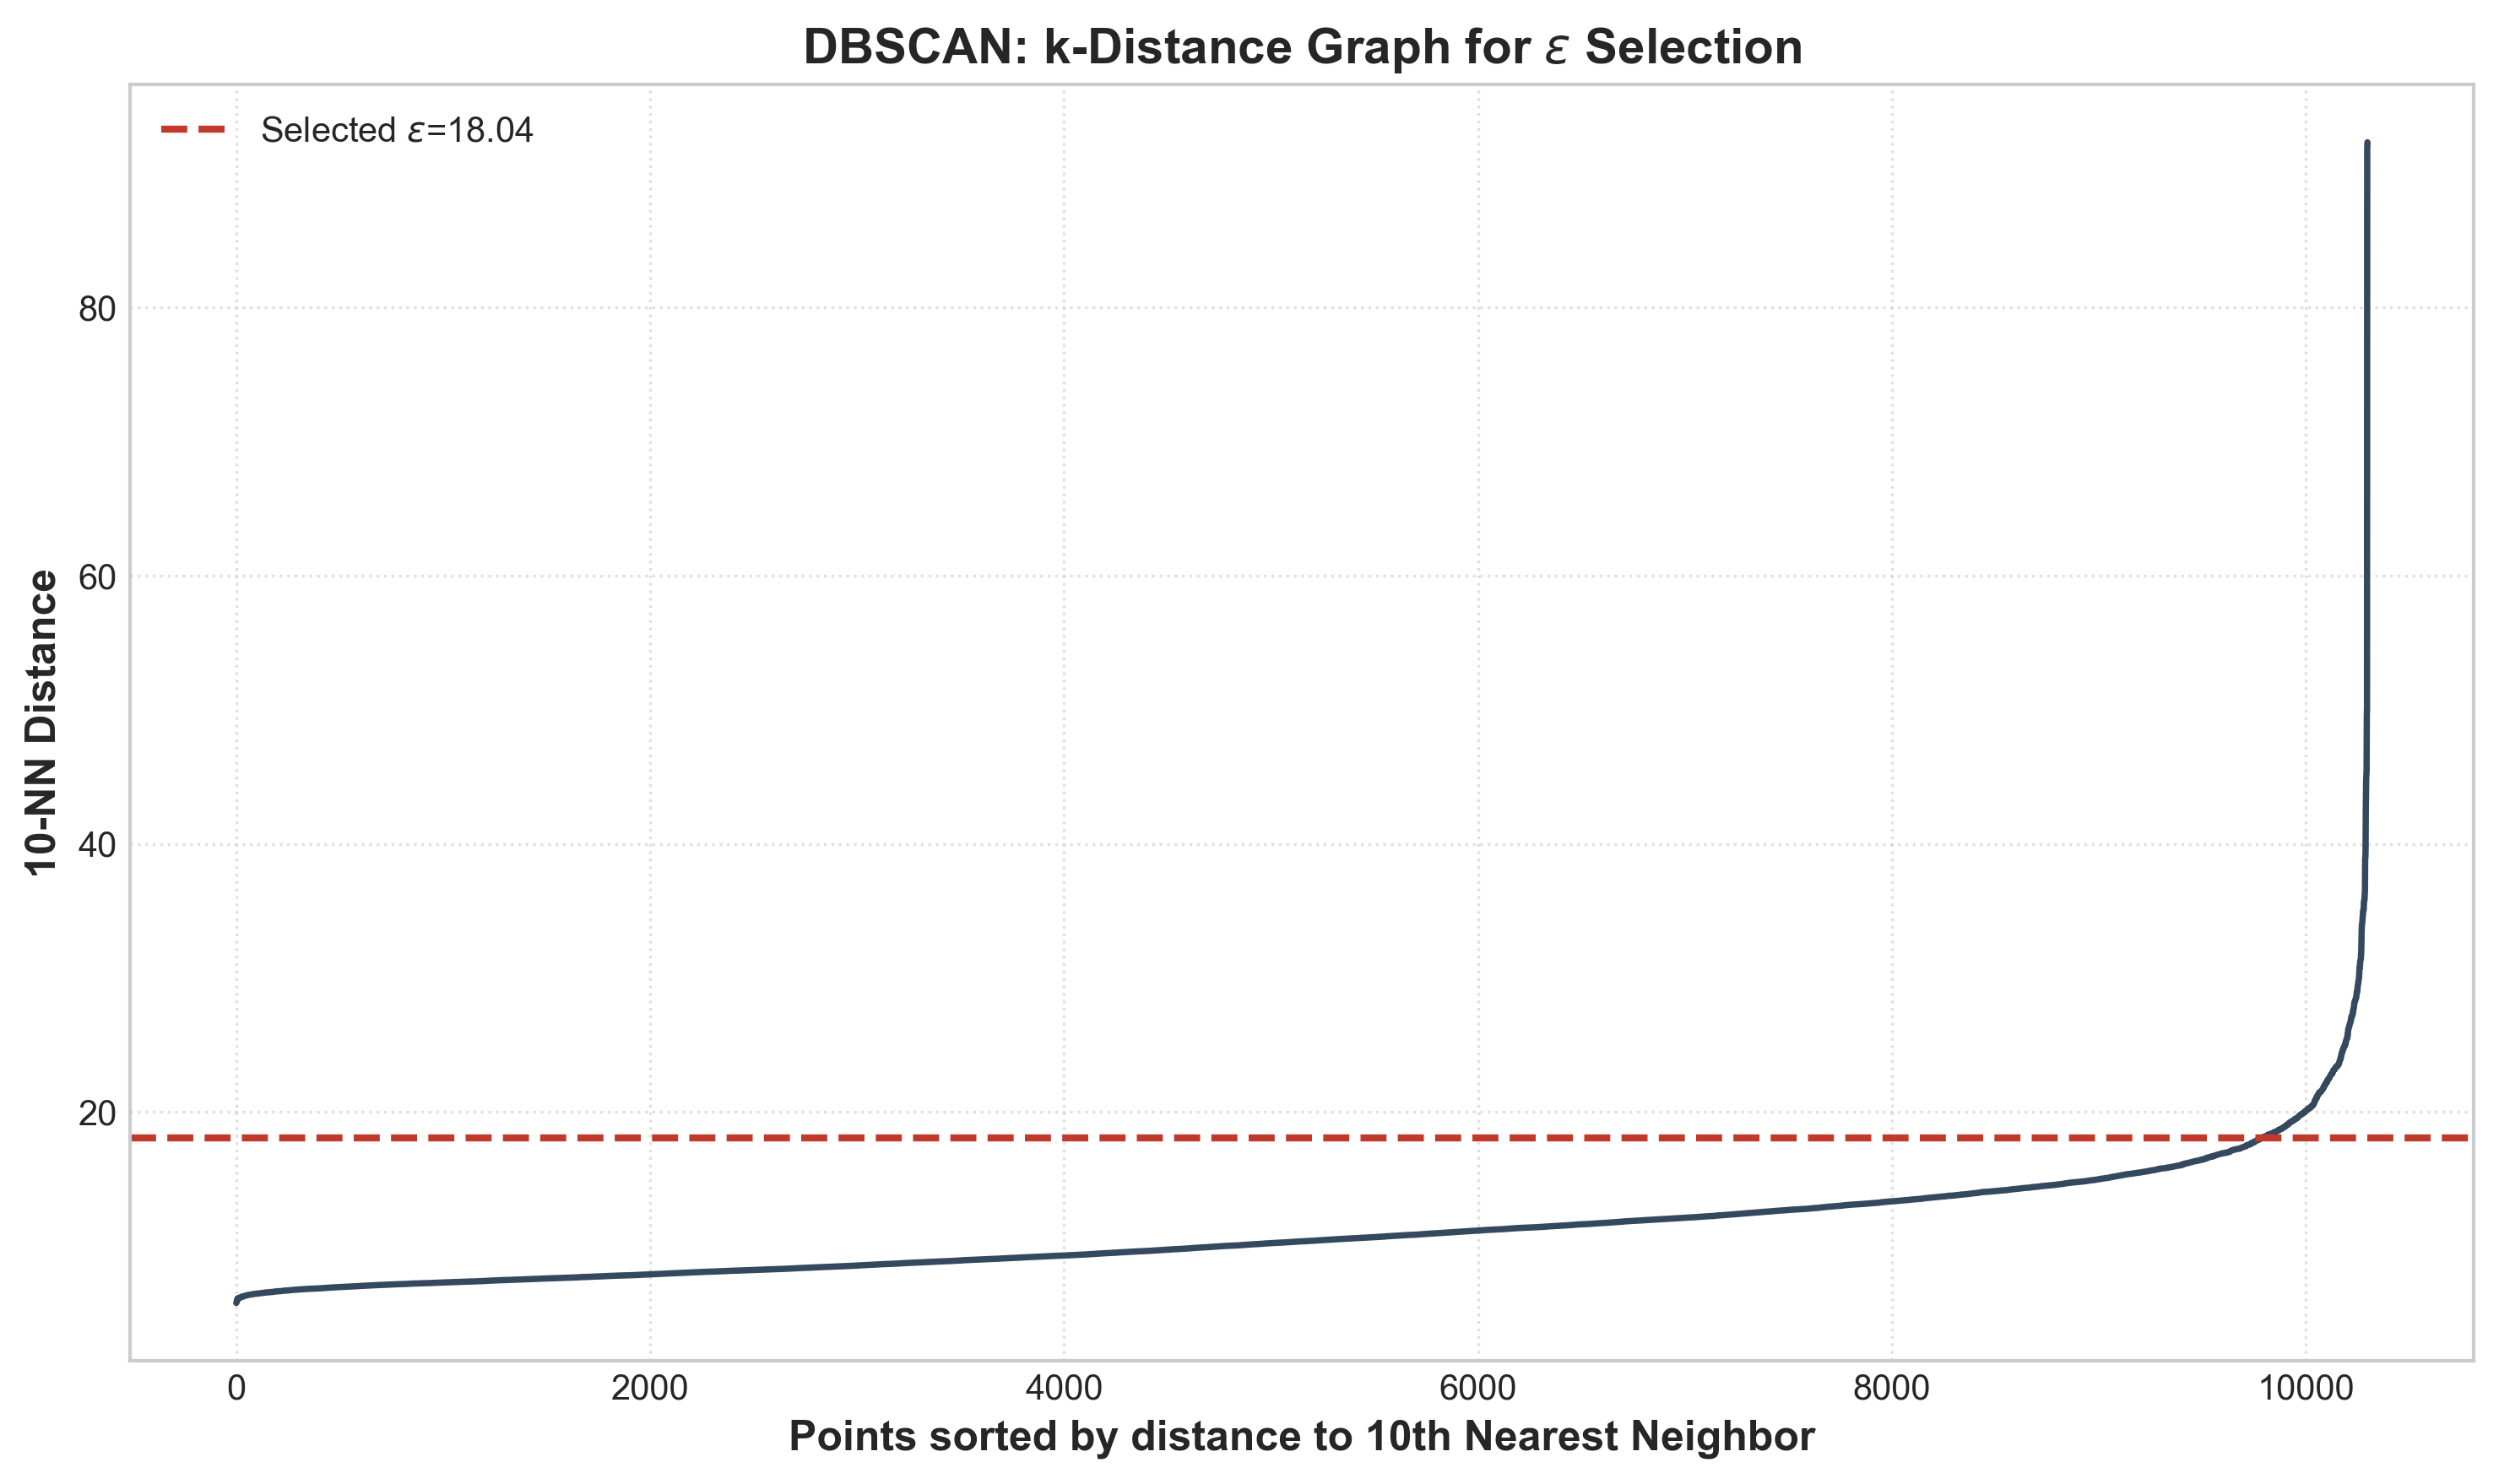
\includegraphics[width=0.75\linewidth]{04_dbscan_kdistance_graph.png}
\caption{DBSCAN k-Distance Graph used for $\epsilon$ Selection.}
\label{fig:kdist}
\end{figure}

\begin{table}[H]
\centering
\caption{DBSCAN Grid Search Results (Selected Rows)}
\label{tab:dbscan_grid}
\resizebox{\linewidth}{!}{
\begin{tabular}{ccccccc}
\toprule
\textbf{$\epsilon$} & \textbf{minPts} & \textbf{Clusters} & \textbf{Noise \%} & \textbf{Silhouette} & \textbf{ARI} & \textbf{NMI} \\
\midrule
13.68 & 5 & 11 & 9.0\% & $-0.0137$ & 0.0212 & 0.0806 \\
14.50 & 15 & 2 & 9.1\% & 0.3551 & 0.0206 & 0.0720 \\
15.66 & 10 & 3 & 5.3\% & 0.3122 & 0.0102 & 0.0524 \\
16.35 & 5 & 2 & 3.3\% & 0.3698 & 0.0046 & 0.0259 \\
\textbf{18.04} & \textbf{5} & \textbf{2} & \textbf{2.2\%} & \textbf{0.4091 (Best)} & 0.0027 & 0.0191 \\
18.04 & 10 & 1 & 2.6\% & N/A & 0.0035 & 0.0220 \\
\bottomrule
\end{tabular}
}
\end{table}

\noindent
\textbf{Selected Configuration:} $\epsilon=18.04$, minPts=5 (highest Silhouette Score among configurations with $\ge 2$ clusters and noise $< 50\%$). Even at its best internal-validity configuration, DBSCAN converges to the same coarse 2-cluster (dynamic vs. static) structure as K-Means, but with far lower external agreement (ARI=0.0027) — ambiguous boundary points are relabeled as noise rather than assigned to a third meaningful group. Lower $\epsilon$ fragments the dense static-activity region into spurious micro-clusters (row 1: 11 clusters, negative Silhouette).

\begin{figure}[H]
\centering
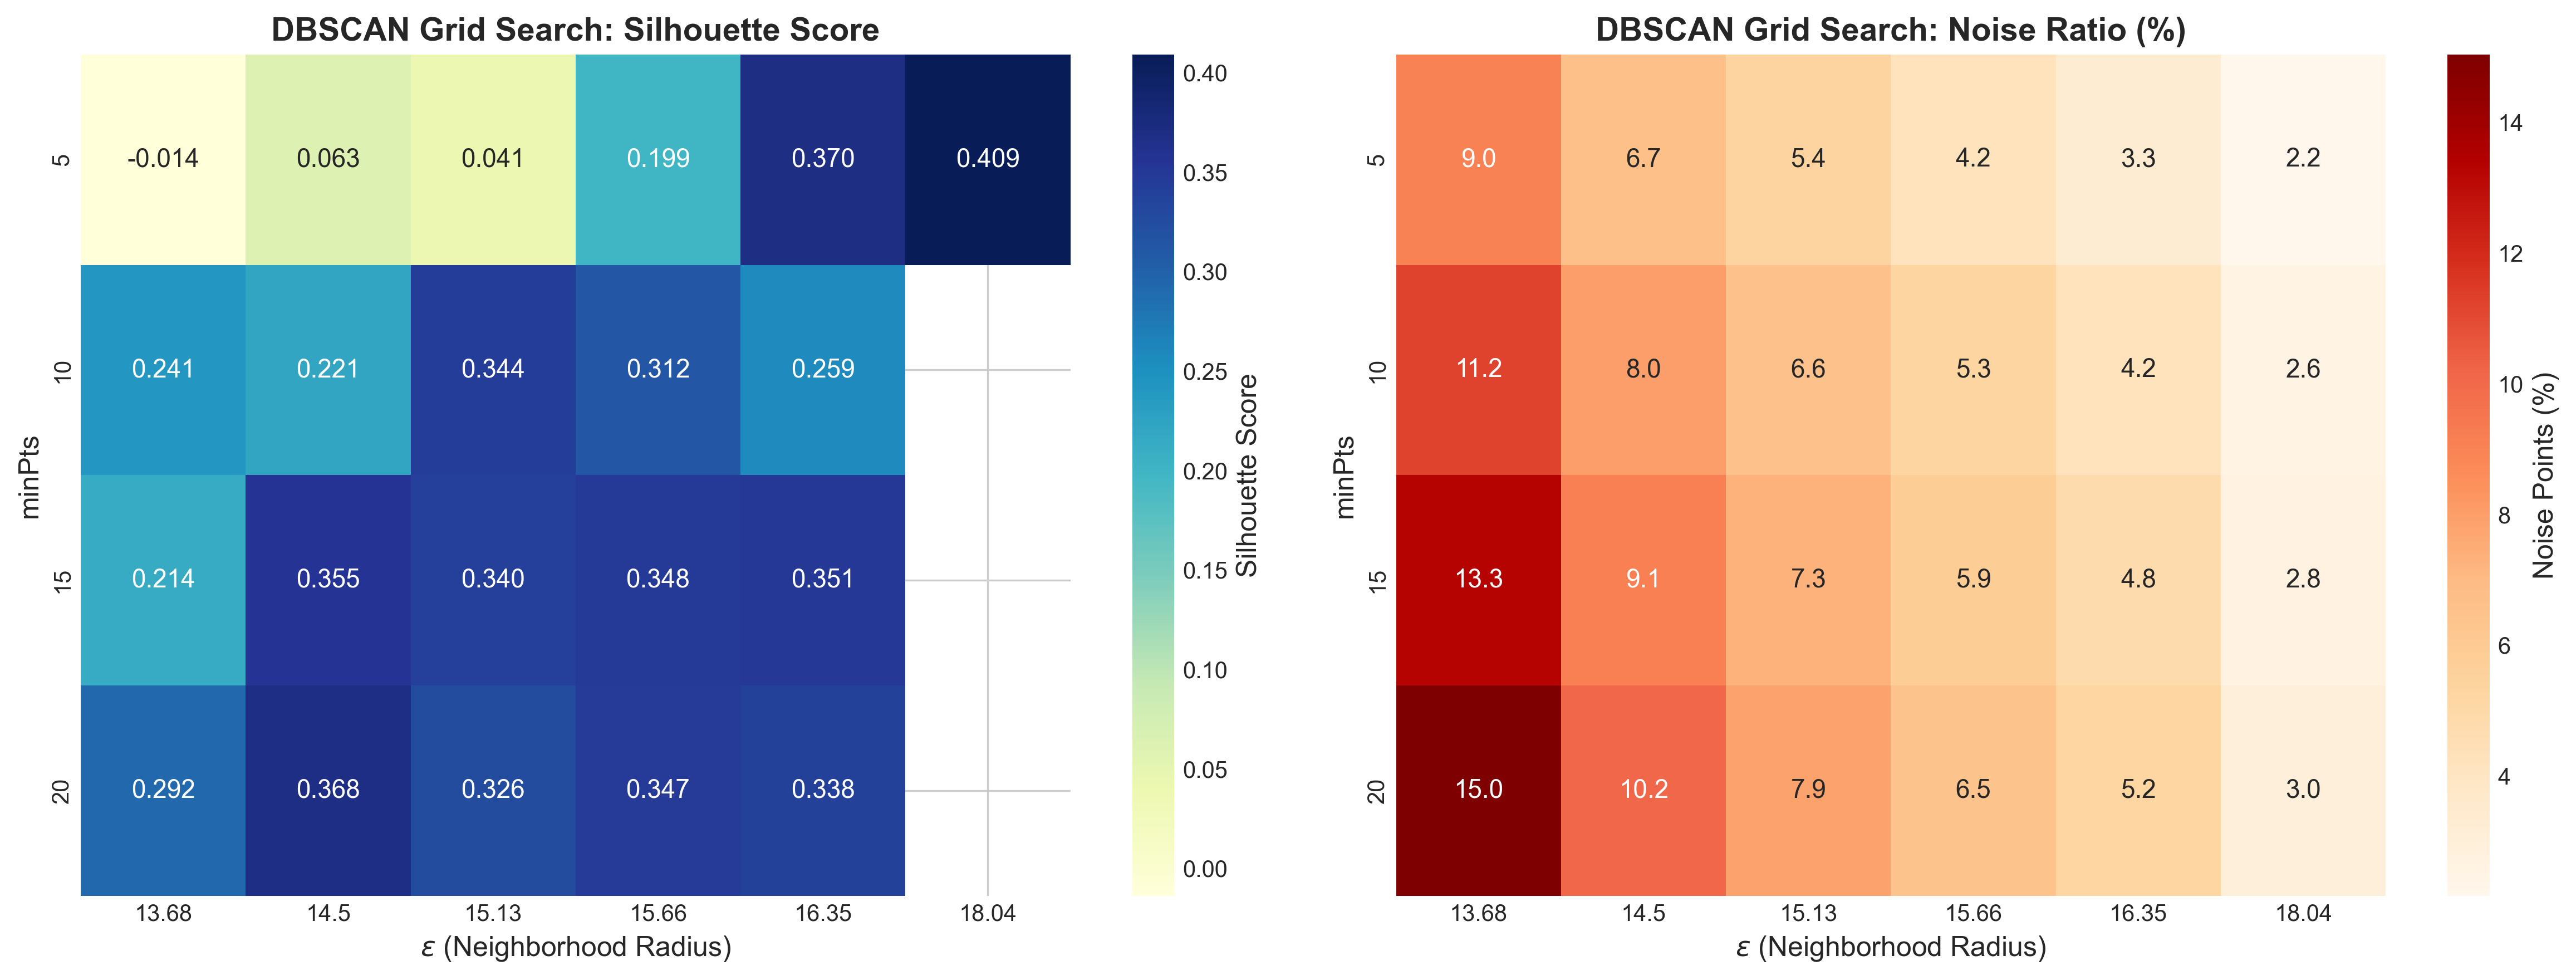
\includegraphics[width=0.98\linewidth]{05_dbscan_grid_search_heatmaps.png}
\caption{DBSCAN ($\epsilon$, minPts) Grid Search: Silhouette Score and Noise Ratio Heatmaps.}
\end{figure}

\section{Model C: Hierarchical Agglomerative Clustering}
Given the $O(n^2)$ memory/time complexity of agglomerative clustering, a stratified random subsample of $n=2{,}497$ points (proportional to class balance) was used for linkage comparison, dendrogram plotting, and HAC metric computation.

\begin{table}[H]
\centering
\caption{Hierarchical Clustering — Linkage Comparison ($k=6$, subsample $n=2{,}497$)}
\label{tab:hac_linkage}
\resizebox{\linewidth}{!}{
\begin{tabular}{lccccc}
\toprule
\textbf{Linkage} & \textbf{Silhouette} & \textbf{Davies-Bouldin} & \textbf{Calinski-Harabasz} & \textbf{ARI} & \textbf{NMI} \\
\midrule
Single & \textbf{0.5539} (degenerate) & 0.2836 & 12.9 & 0.0003 & 0.0044 \\
Complete & 0.3636 & 1.5831 & 630.8 & 0.3253 & 0.5298 \\
Average & 0.3450 (degenerate) & 1.1470 & 57.8 & 0.0031 & 0.0346 \\
\textbf{Ward (Primary)} & 0.1585 & 2.2087 & \textbf{776.6} & \textbf{0.3048} & \textbf{0.4755} \\
\bottomrule
\end{tabular}
}
\end{table}

\noindent
\textbf{Key Finding:} Raw Silhouette Score is misleading here — Single and Average linkage score deceptively high because a near-degenerate solution (one giant cluster plus a handful of outlier singletons) is trivially compact. \textbf{Ward's linkage}, used as the primary configuration per the assignment specification, produces the most structurally meaningful and activity-aligned partition (highest Calinski-Harabasz Index; second-highest ARI/NMI among all linkages), consistent with its minimum-variance merging objective.

\begin{figure}[H]
\centering
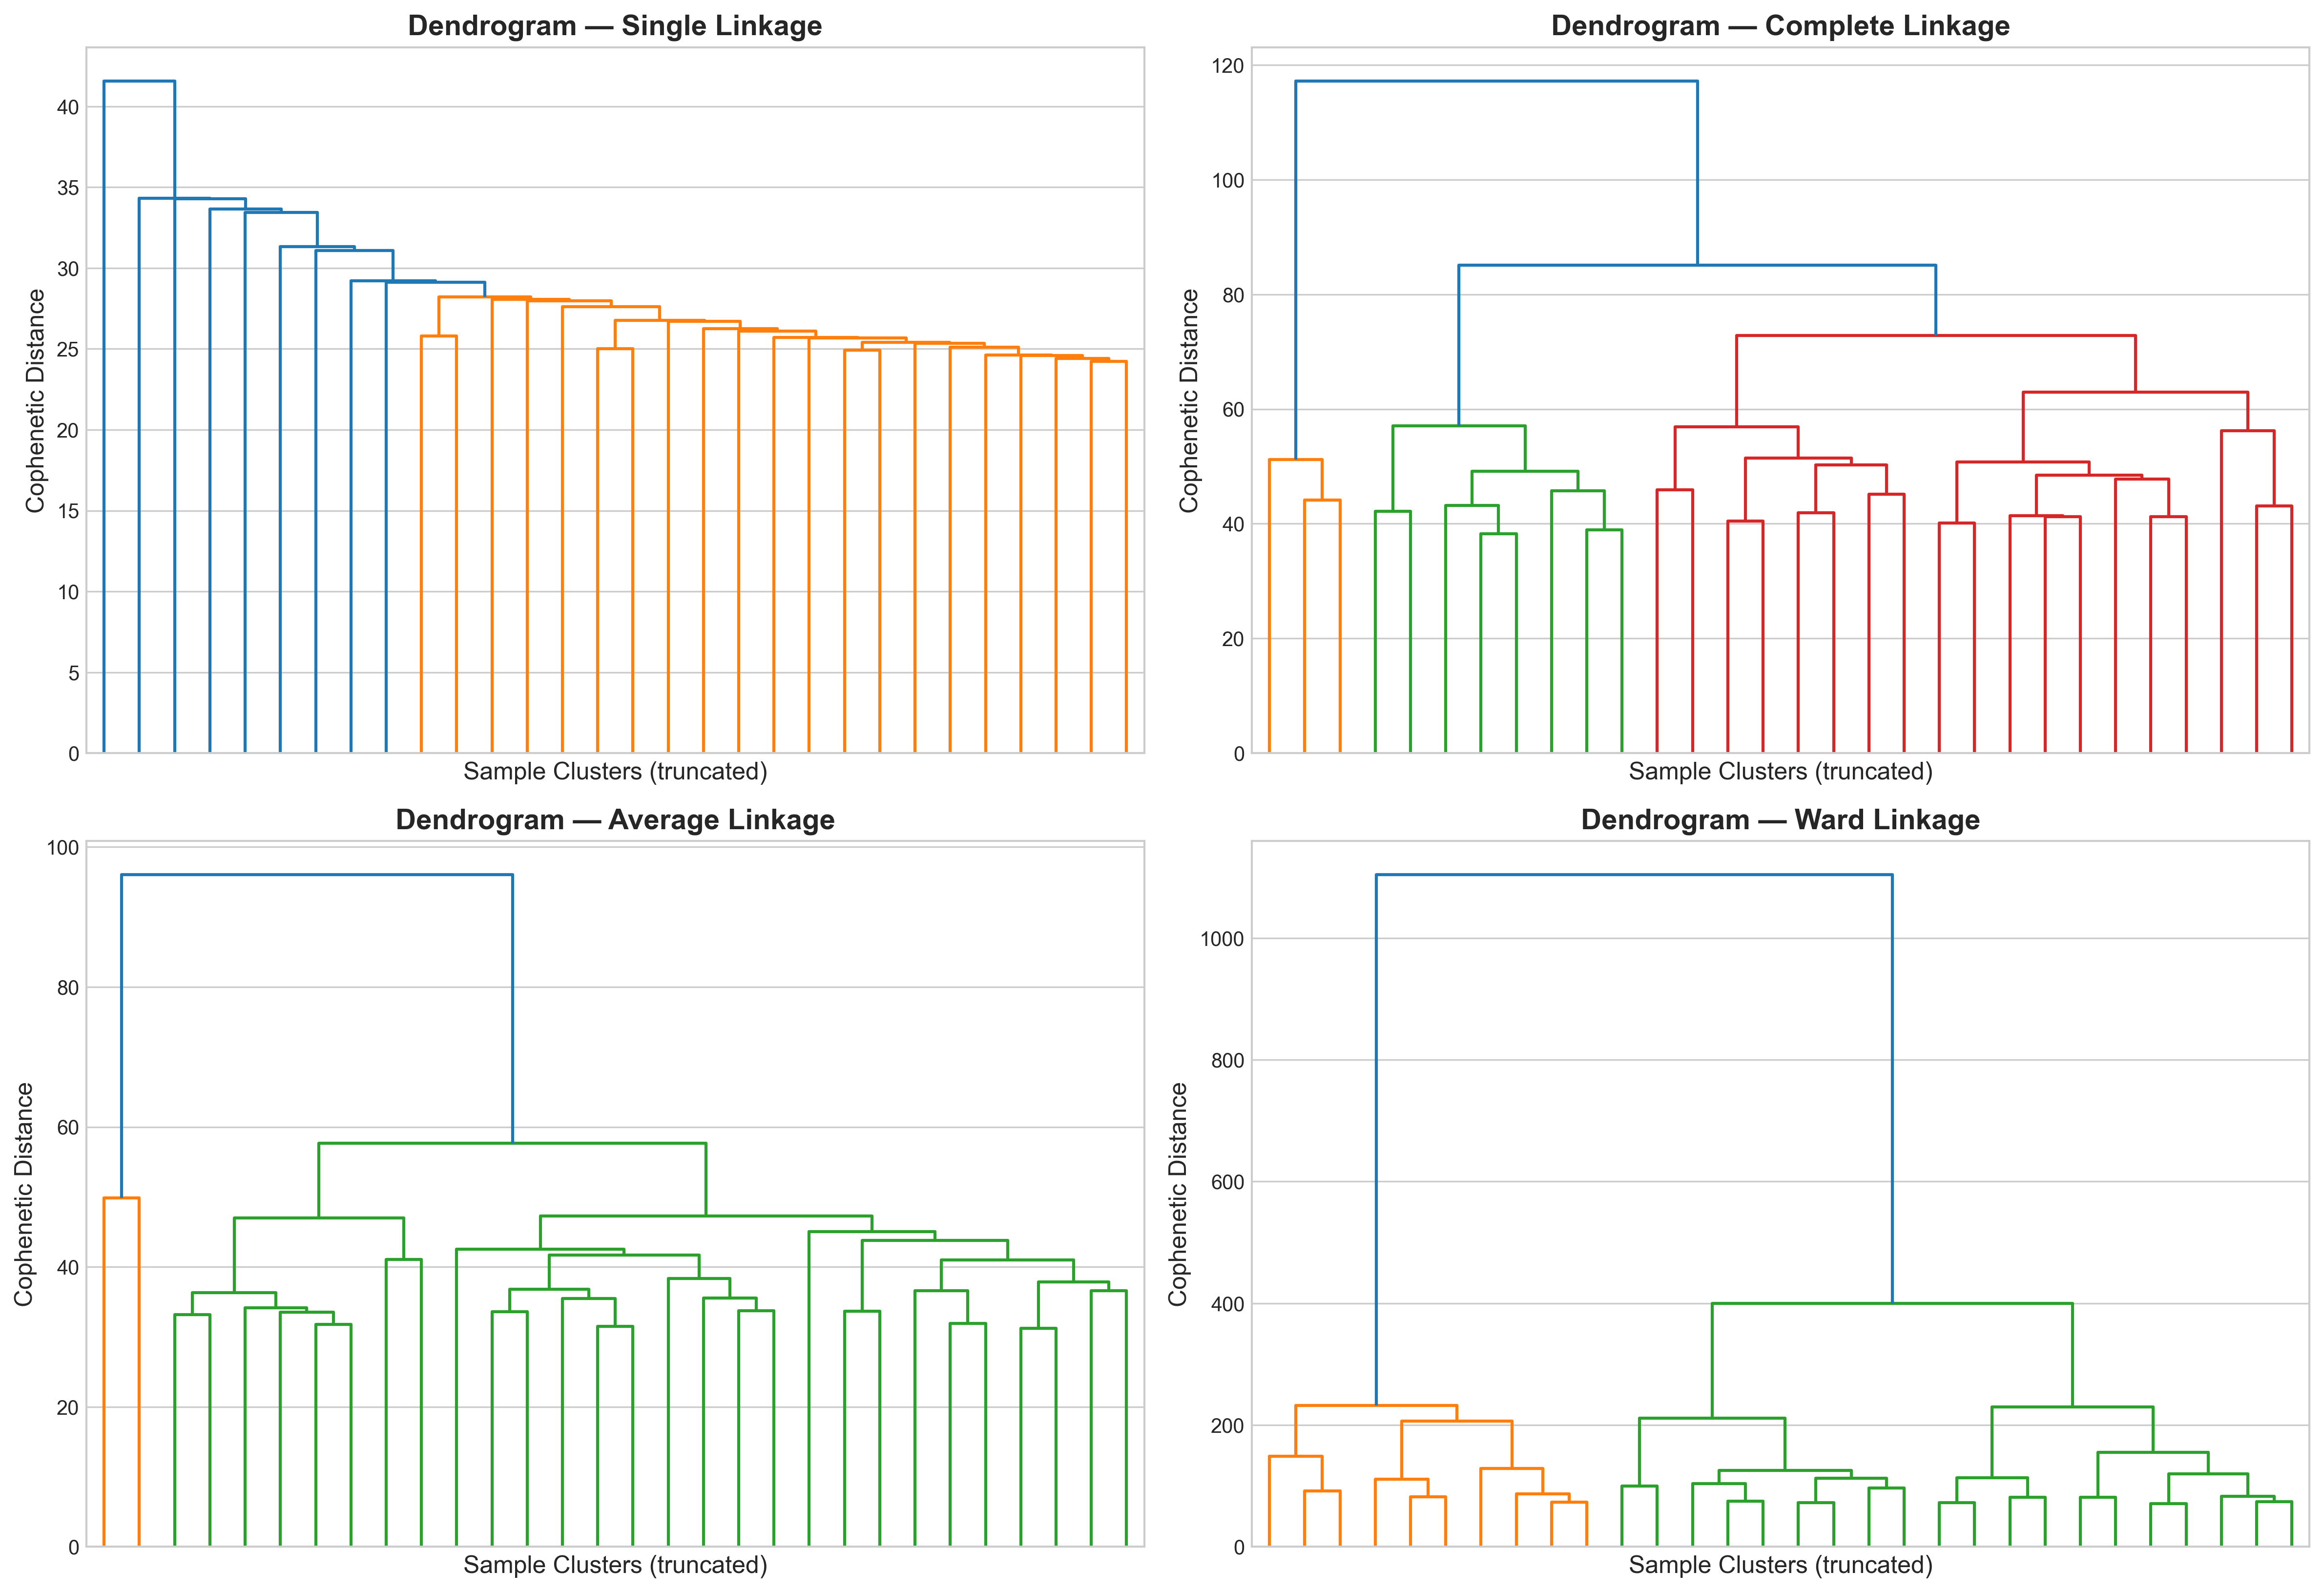
\includegraphics[width=0.98\linewidth]{06_dendrograms_linkage_comparison.png}
\caption{Dendrograms for Single, Complete, Average, and Ward Linkage (truncated to last 30 merges).}
\end{figure}

\section{Cluster Visualization}
Figure~\ref{fig:pca2d} shows the ground-truth activity labels alongside K-Means and DBSCAN cluster assignments projected onto the first two principal components; Figure~\ref{fig:hac2d} shows the HAC subsample similarly; Figure~\ref{fig:tsne} shows a t-SNE projection (subsample $n=3{,}000$) for non-linear visual validation.

\begin{figure}[H]
\centering
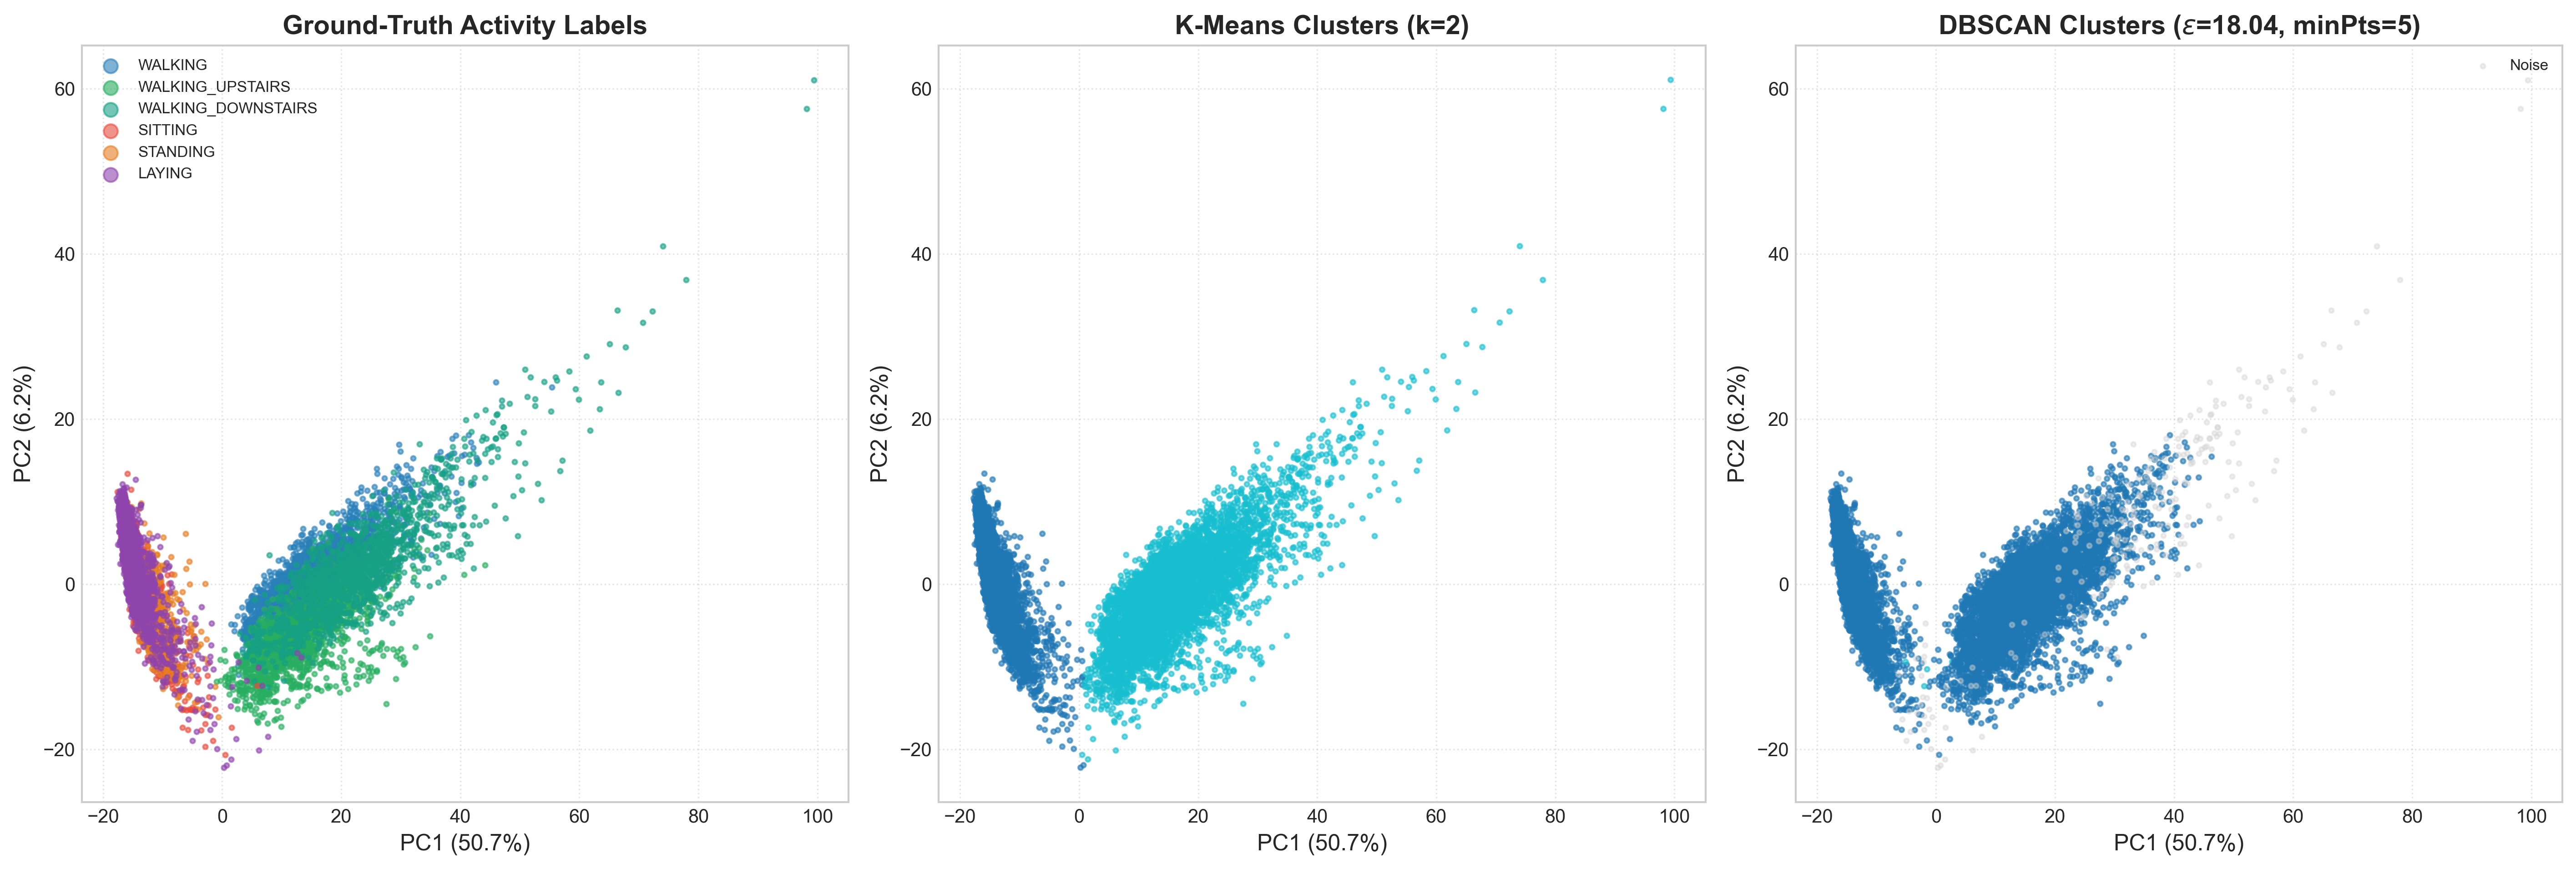
\includegraphics[width=0.98\linewidth]{07_pca_2d_cluster_scatter.png}
\caption{PCA 2D Projection: Ground-Truth Labels vs K-Means (k=2) vs DBSCAN Clusters.}
\label{fig:pca2d}
\end{figure}

\begin{figure}[H]
\centering
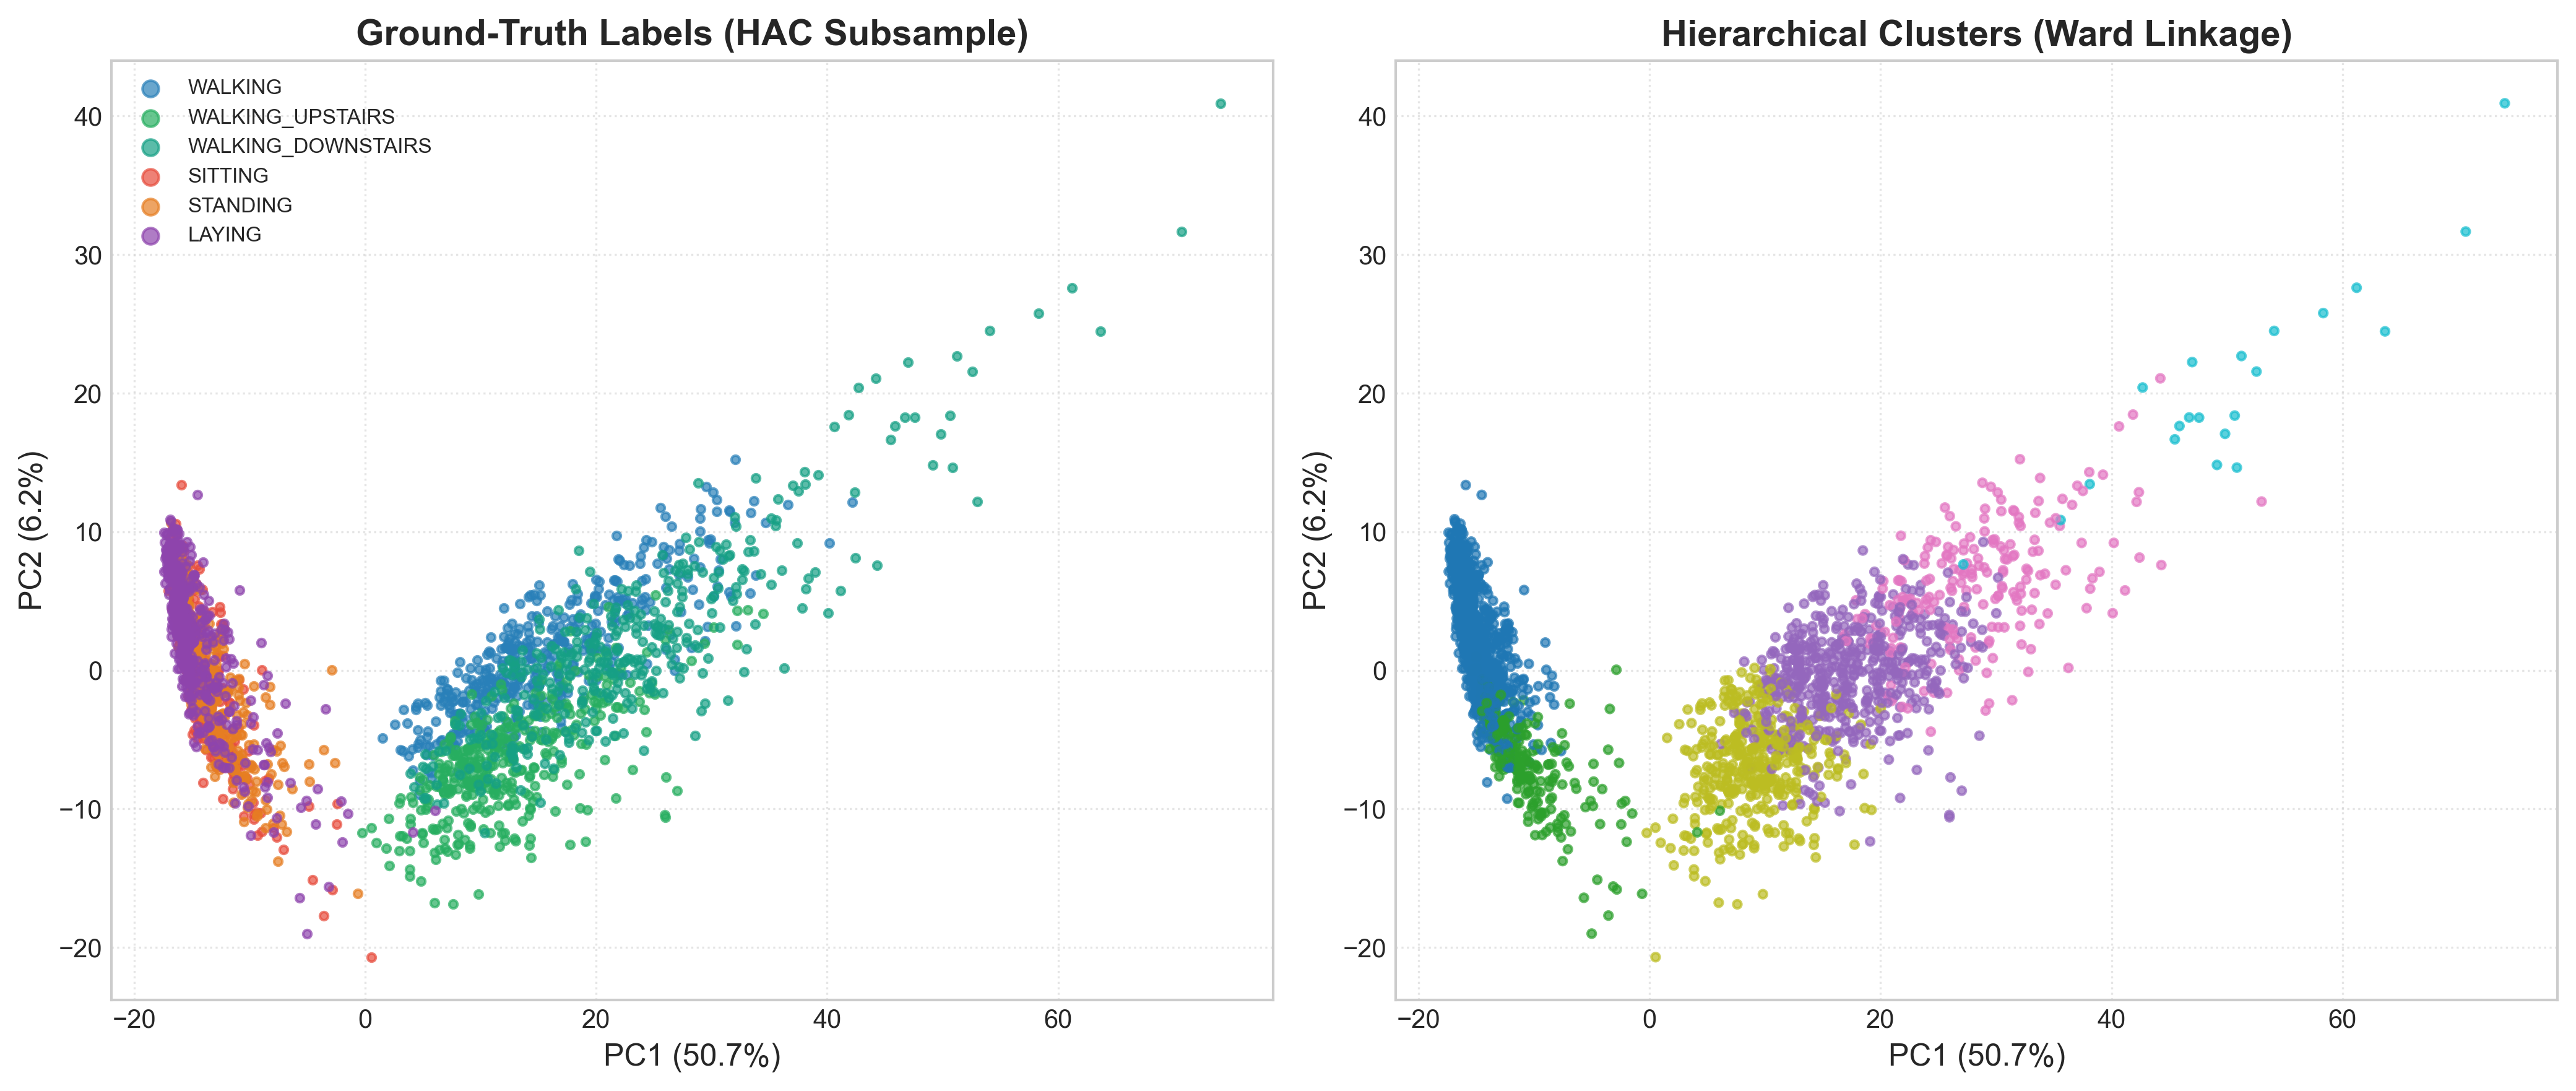
\includegraphics[width=0.85\linewidth]{08_hac_pca_2d_cluster_scatter.png}
\caption{PCA 2D Projection (HAC Subsample): Ground-Truth Labels vs Ward-Linkage Clusters.}
\label{fig:hac2d}
\end{figure}

\begin{figure}[H]
\centering
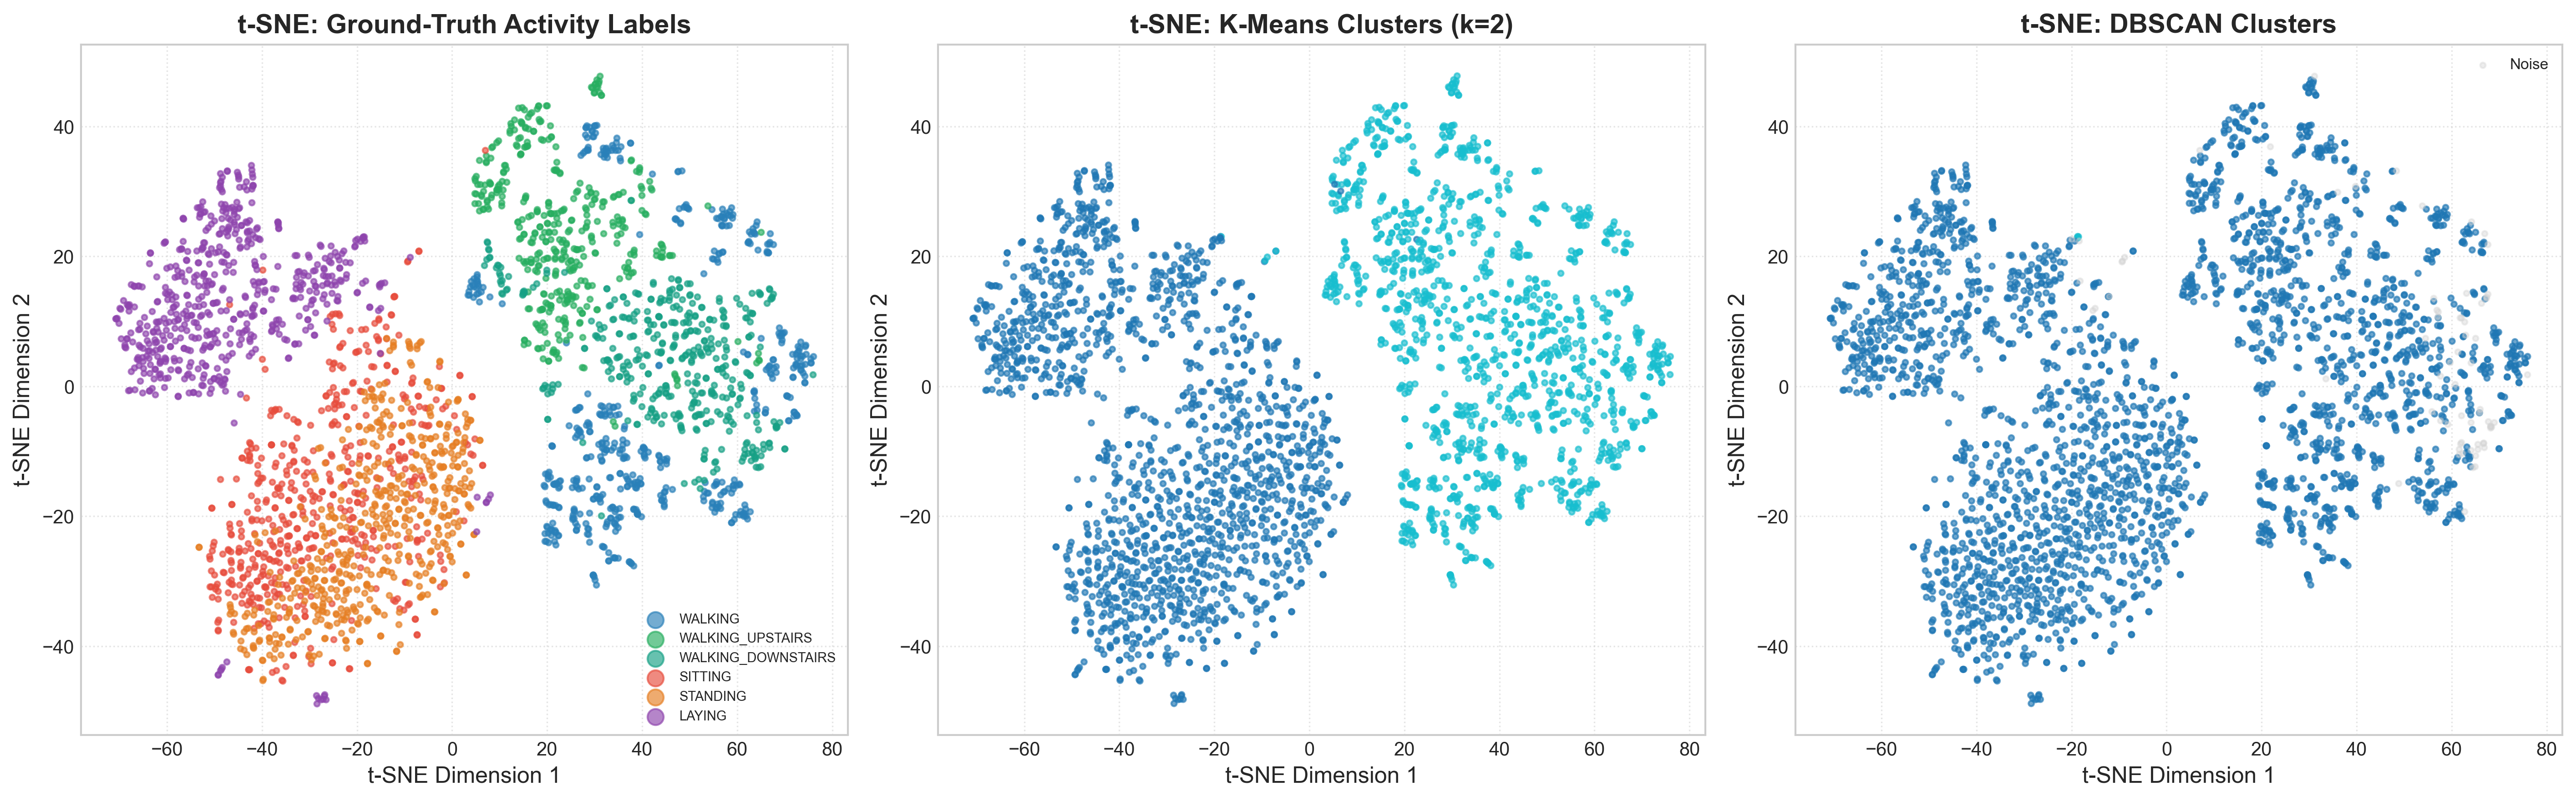
\includegraphics[width=0.98\linewidth]{09_tsne_cluster_comparison.png}
\caption{t-SNE 2D Projection: Ground-Truth Labels vs K-Means vs DBSCAN (subsample $n=3{,}000$).}
\label{fig:tsne}
\end{figure}

\section{Evaluation Metrics \& Cross-Algorithm Comparison}

\begin{table}[H]
\centering
\caption{Cross-Algorithm Internal \& External Validation Summary}
\label{tab:cross_algo}
\resizebox{\linewidth}{!}{
\begin{tabular}{lcccccc}
\toprule
\textbf{Algorithm} & \textbf{Config} & \textbf{Silhouette} & \textbf{Davies-Bouldin} & \textbf{Calinski-Harabasz} & \textbf{ARI} & \textbf{NMI} \\
\midrule
\textbf{K-Means} & k=2 & \textbf{0.4366} & \textbf{0.9611} & \textbf{9560.0} & 0.3296 & \textbf{0.5455} \\
\textbf{DBSCAN} & $\epsilon$=18.04, mp=5 & 0.4091 & N/A & N/A & 0.0027 & 0.0191 \\
\textbf{Hierarchical (Ward)} & 6 clusters & 0.1585 & 2.2087 & 776.6 & 0.3048 & 0.4755 \\
\bottomrule
\end{tabular}
}
\end{table}

\begin{figure}[H]
\centering
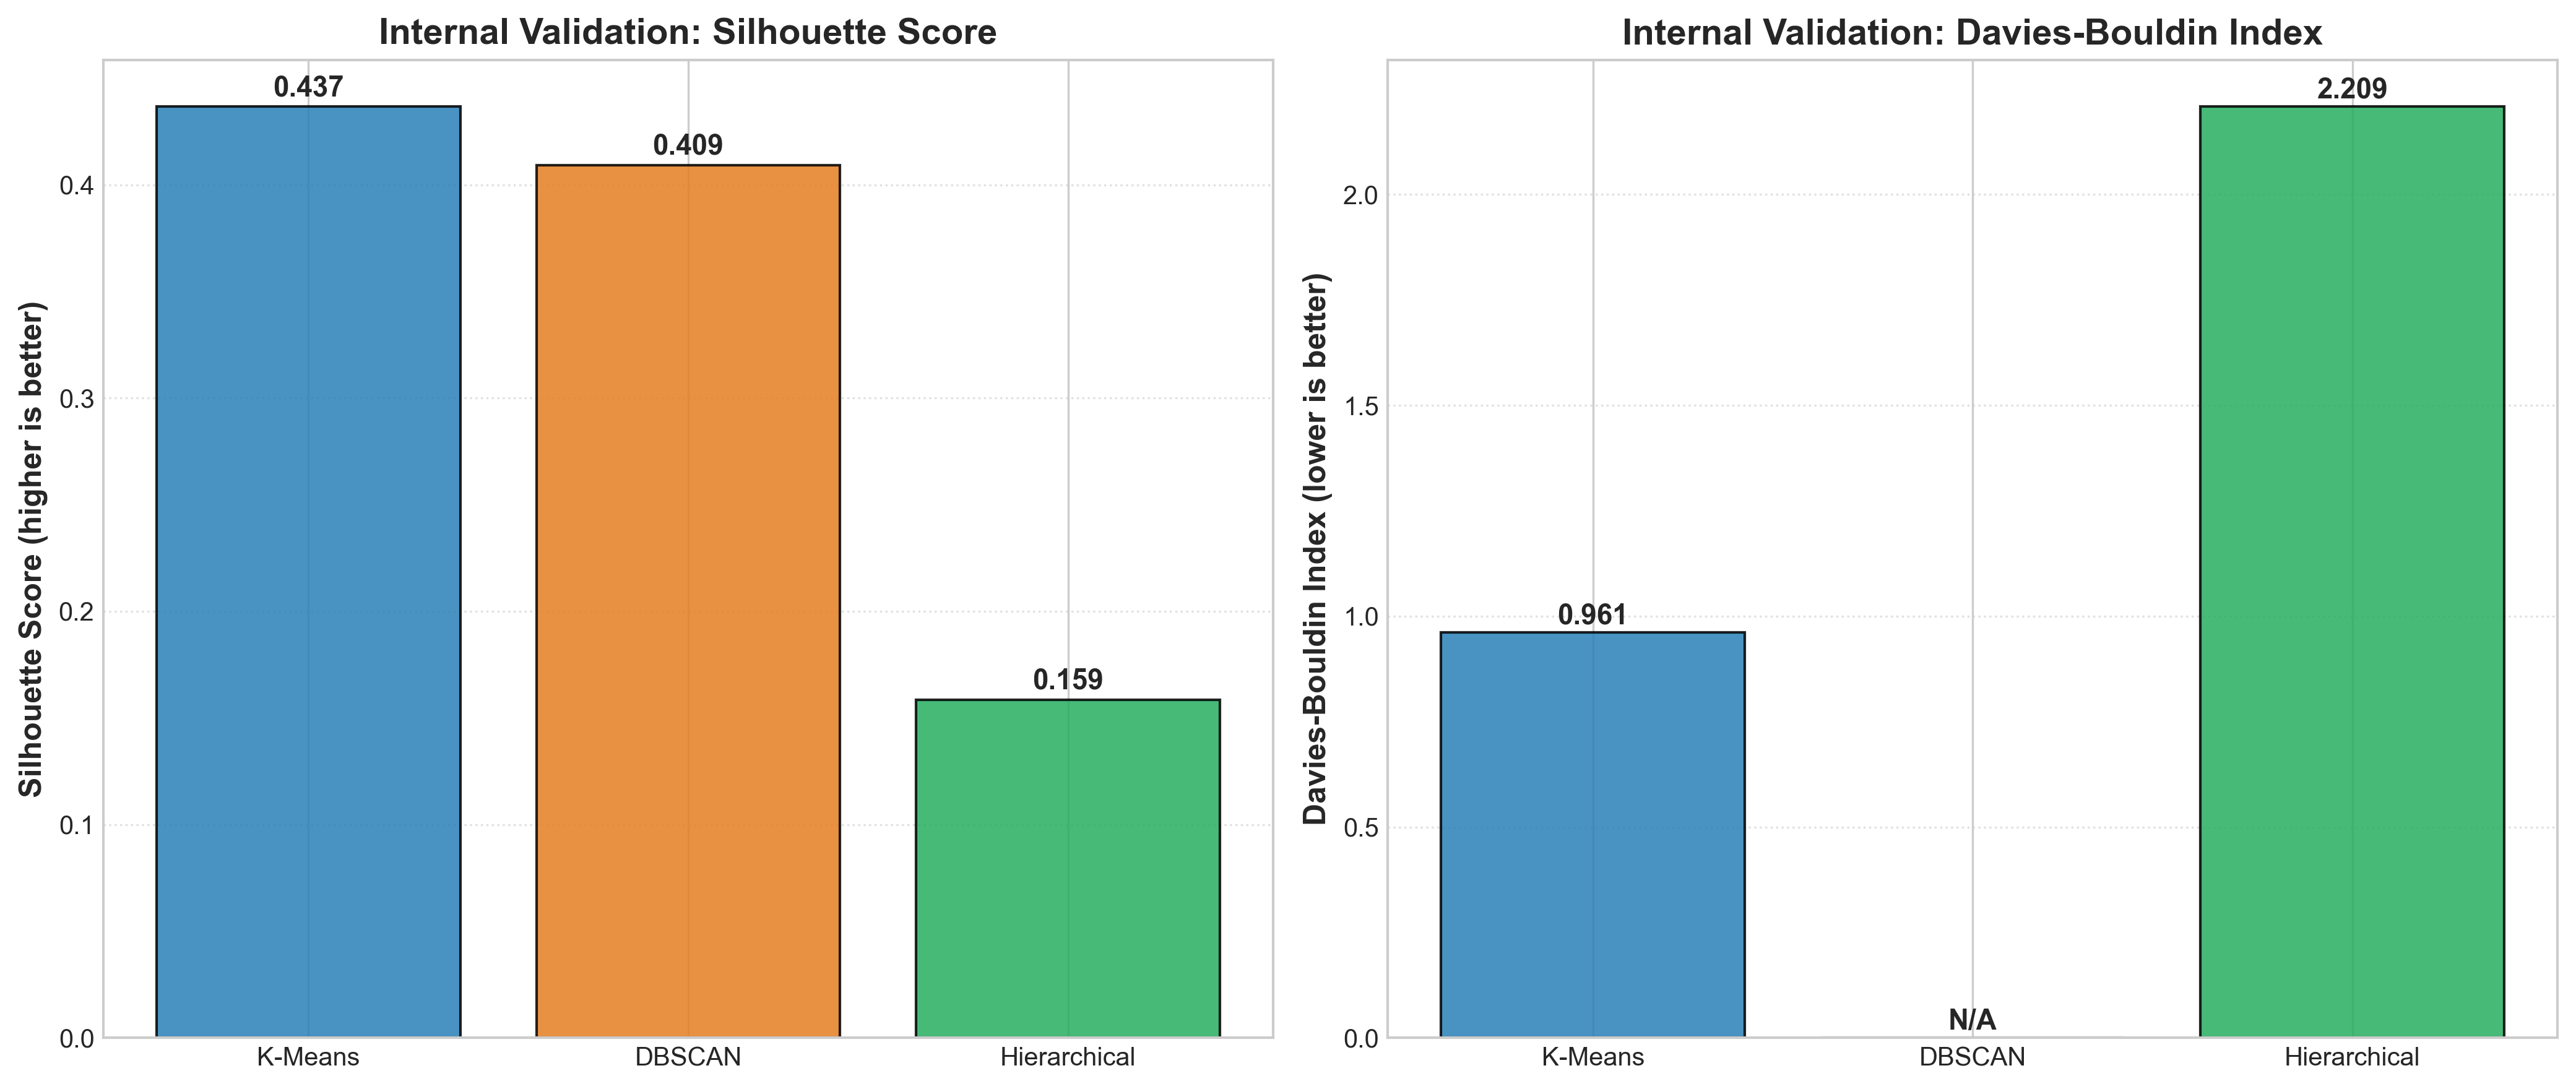
\includegraphics[width=0.98\linewidth]{10_internal_metrics_comparison.png}
\caption{Internal Validation Metrics Comparison: Silhouette Score and Davies-Bouldin Index.}
\end{figure}

\begin{figure}[H]
\centering
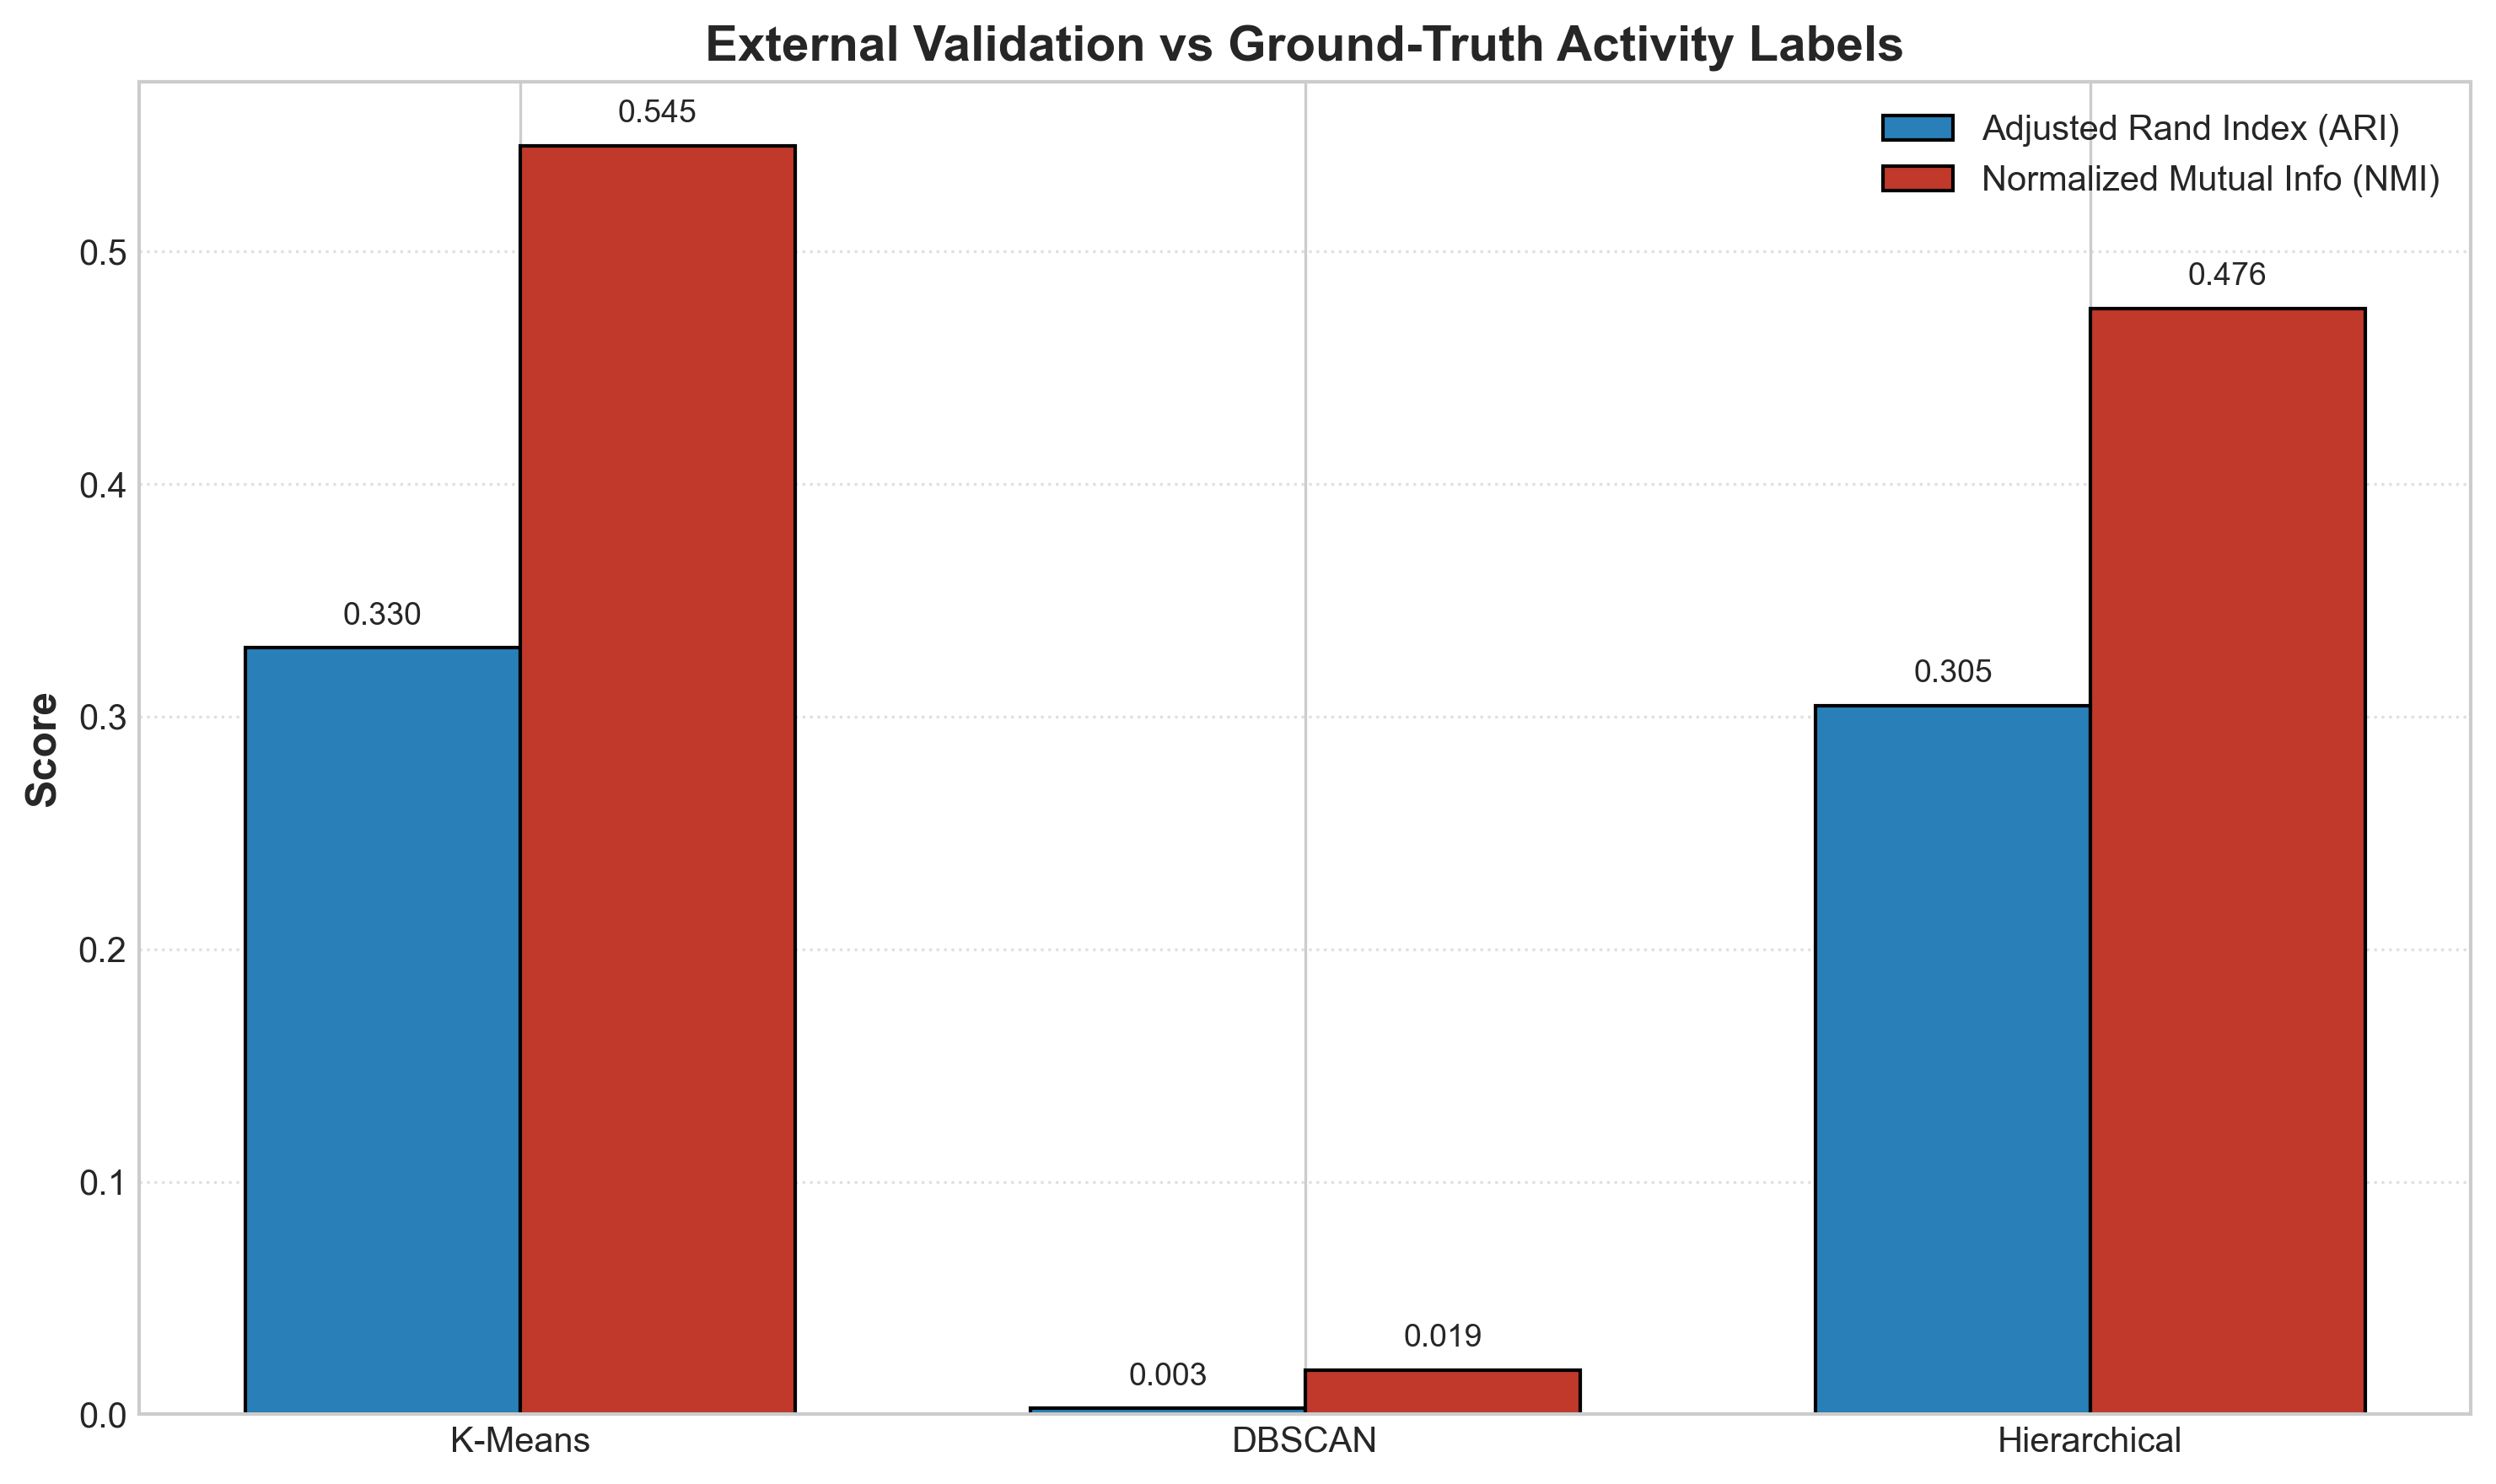
\includegraphics[width=0.85\linewidth]{11_external_metrics_comparison.png}
\caption{External Validation Metrics Comparison: Adjusted Rand Index and Normalized Mutual Information.}
\end{figure}

\begin{figure}[H]
\centering
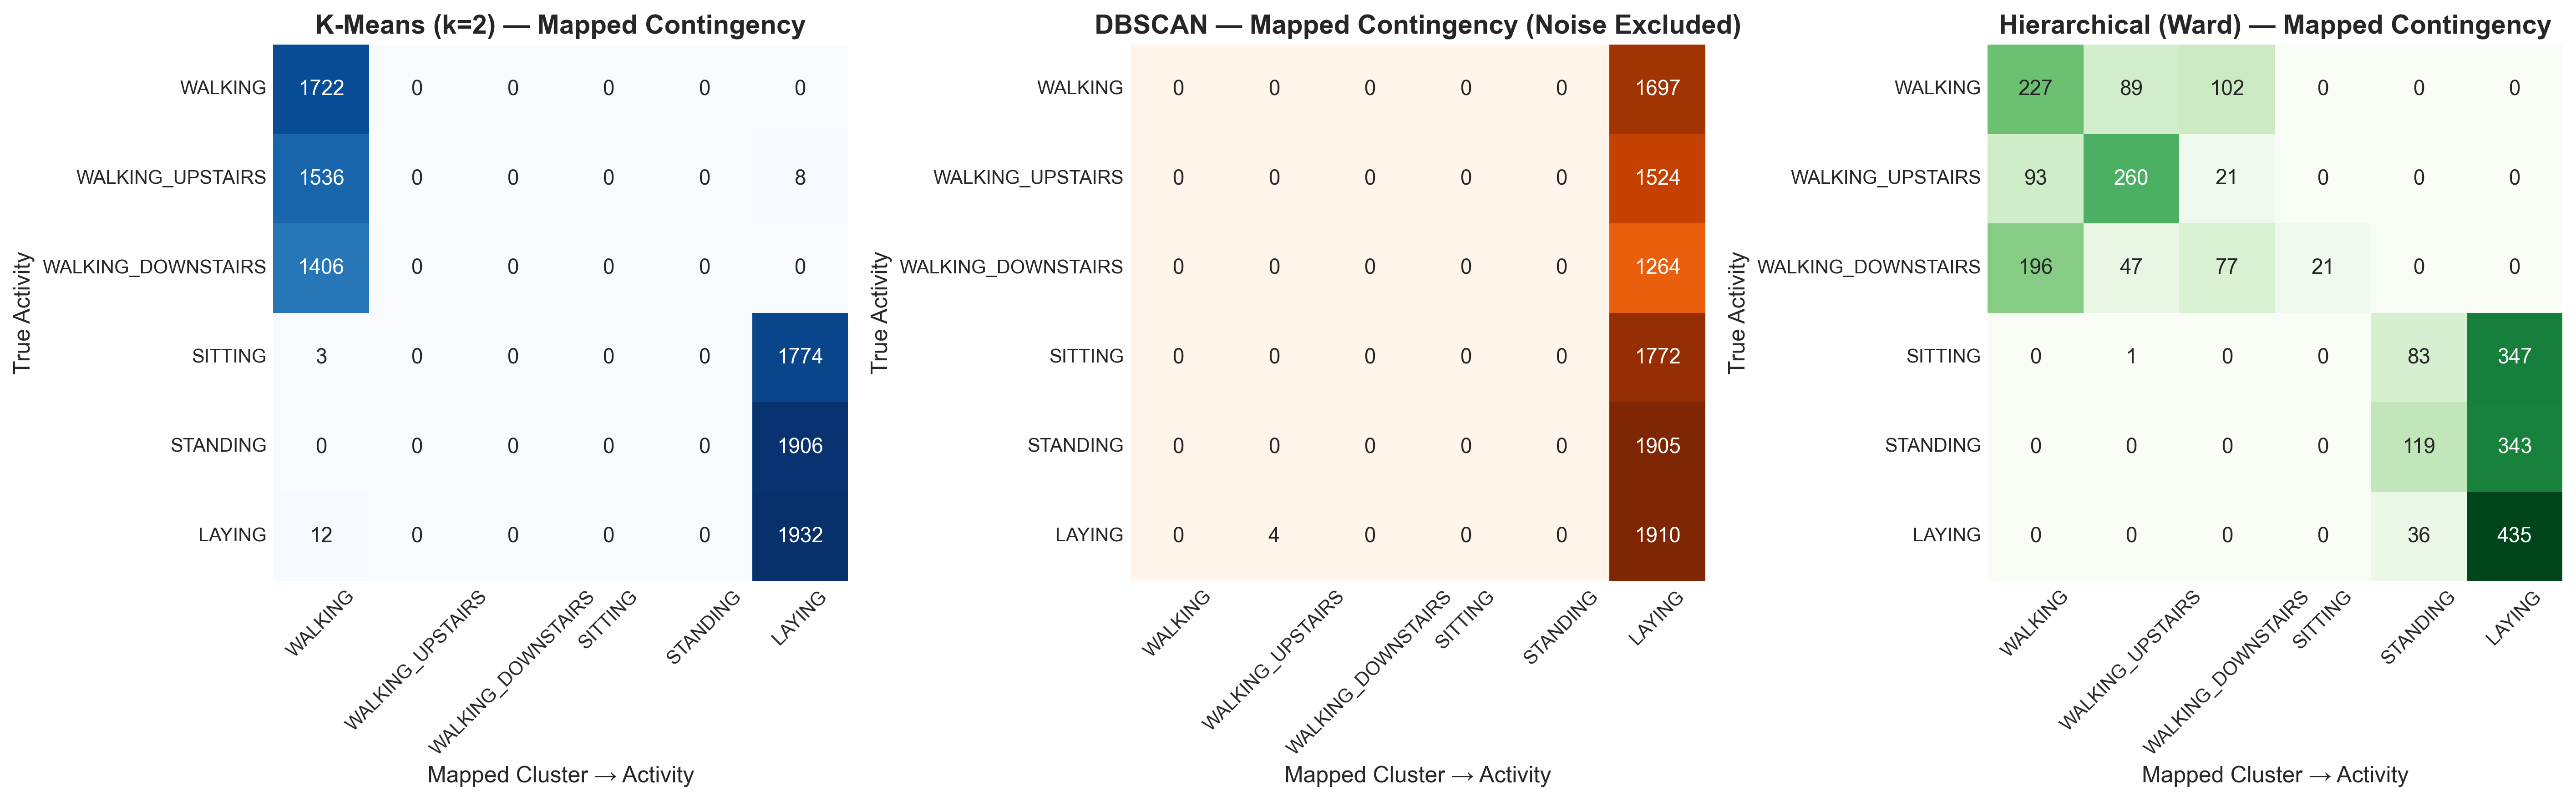
\includegraphics[width=0.98\linewidth]{12_cluster_activity_contingency.png}
\caption{Cluster-to-Activity Contingency Heatmaps (Majority-Vote Mapped) for K-Means, DBSCAN, and Hierarchical (Ward).}
\end{figure}

\section{Answers to Observation Questions \& Detailed Discussion}

\subsection{1. Which algorithm produced the most meaningful clusters? Why?}
\textbf{K-Means (k=2)} produced the most internally \textit{and} externally valid clustering overall — highest Silhouette (0.4366), lowest Davies-Bouldin (0.9611), highest Calinski-Harabasz (9560.0), and the best external agreement (ARI=0.3296, NMI=0.5455). Its centroid-based partitioning naturally captures the dominant, near-linearly-separable dynamic-vs-static split along PC1 (50.7\% variance). \textbf{Hierarchical Clustering with Ward linkage} is preferable when finer-grained activity resolution is needed, trading internal compactness for a partition that still meaningfully separates most activity pairs. \textbf{DBSCAN} was the least meaningful: its respectable Silhouette Score (0.4091) is an artifact of finding the same coarse 2-cluster split as K-Means while relabeling ambiguous boundary points as noise; its external agreement (ARI=0.0027) is essentially at chance level.

\subsection{2. How sensitive was K-Means to the choice of k?}
Highly sensitive, revealing a genuine tension between internal and external validity. WCSS shows no elbow and Silhouette peaks sharply at $k=2$, implying the internally "correct" answer is a 2-cluster dynamic-vs-static split. Yet ARI/NMI against the true 6-activity labels \textit{improve} as $k$ increases from 2 to 6--8 (ARI: $0.330 \to 0.420$--$0.431$), because larger $k$ progressively resolves individual activities nested within each super-cluster. Internal cluster-validity metrics and external label-agreement metrics can disagree substantially, and the "right" $k$ depends on the downstream goal.

\subsection{3. Did DBSCAN detect noise or small clusters effectively?}
Partially. The k-distance-guided $\epsilon$ selection identified a low, stable noise fraction (2.2\% at the best configuration) — genuinely sparse/boundary points were correctly flagged rather than forced into a cluster. However, DBSCAN was \textit{not} effective at detecting small, meaningful activity-level clusters: at low $\epsilon$ it fragmented the dense static-activity region into spurious micro-clusters (11 clusters at $\epsilon=13.68$, with a negative Silhouette Score), while at higher $\epsilon$ it collapsed to the same trivial 2-cluster split as K-Means. This reflects that the HAR feature manifold is a continuum of varying local density (SITTING/STANDING/LAYING densely overlap) rather than well-separated, uniform-density blobs.

\subsection{4. How does linkage choice (single/complete/ward) affect hierarchical clustering?}
Dramatically. \textbf{Single linkage} is highly susceptible to \textit{chaining}: closely-spaced point sequences bridge otherwise distinct activity groups, producing one dominant cluster and several near-empty singletons. \textbf{Average linkage} showed the same pathology. Both scored deceptively high raw Silhouette (0.55 and 0.35) purely because a near-single-cluster solution is trivially compact, yet ARI/NMI were near zero. \textbf{Complete} and \textbf{Ward} linkage both resisted chaining and produced balanced, activity-aligned partitions; Ward achieved the highest Calinski-Harabasz Index (776.6) and the best overall trade-off, justifying its use as the assignment's mandated linkage criterion.

\subsection{5. Which internal metric best matched your visual intuition of cluster quality?}
The \textbf{Calinski-Harabasz Index} best matched visual/PCA-scatter intuition, correctly rewarding Ward linkage (776.6) and K-Means $k=2$ (9560.0) — both visibly compact and well-separated in the PCA scatter plots — without being fooled by the degenerate single/average-linkage chains. \textbf{Silhouette Score}, by contrast, was actively misleading for Hierarchical Clustering (rewarding degenerate chaining), requiring cross-validation against Davies-Bouldin and the external ARI/NMI metrics — reinforcing that internal metrics should always be triangulated with several complementary measures rather than trusted individually.

\section{Conclusion}
This experimental study demonstrates that clustering algorithm choice, hyperparameter selection, and validation metric interpretation are deeply interconnected on real-world sensor data:
\begin{enumerate}
\item \textbf{K-Means} with a low $k$ (2) delivers the most internally coherent partition (dynamic vs. static activity), while a higher $k$ (6--8) better recovers the true activity taxonomy at the cost of internal compactness.
\item \textbf{DBSCAN}'s density-based assumptions are poorly matched to the continuous, overlapping HAR feature manifold; its apparently strong Silhouette Score at the best configuration masks near-chance-level agreement with ground truth (ARI=0.0027).
\item \textbf{Hierarchical Clustering} is highly sensitive to linkage criterion, with Ward's minimum-variance objective clearly outperforming Single/Average linkage's chaining-prone solutions (ARI: 0.3048 vs. $\le 0.0031$).
\item No single internal metric was sufficient in isolation — Silhouette, Davies-Bouldin, and Calinski-Harabasz needed to be interpreted jointly and cross-referenced with external ARI/NMI to reach reliable conclusions about genuine cluster quality.
\item Overall, \textbf{K-Means (k=2)} and \textbf{Hierarchical Clustering (Ward)} both substantially outperformed \textbf{DBSCAN} at recovering the underlying human activity structure from unlabeled smartphone sensor data.
\end{enumerate}

\end{document}
